\documentclass[a4paper]{book}

\usepackage{fullpage} % Package to use full page
\usepackage{parskip} % Package to tweak paragraph skipping
\usepackage{tikz} % Package for drawing
\usepackage{amsmath}
\usepackage{hyperref}
\usepackage[utf8]{inputenc}
\usepackage[x11names]{xcolor}
\usepackage{textcomp}
\colorlet{myGray}{gray!15}

\usepackage[
backend=biber,
style=alphabetic,
sorting=ynt
]{biblatex}
\addbibresource{bibliography.bib}

\newcommand{\Tr}[1]{\mathrm{Tr}\left[{#1}\right]}
\newcommand{\iu}{{i\mkern1mu}}

\renewcommand{\chaptername}{Chapitre}
\renewcommand{\bibname}{Bibliographie}

\title{Optique des lasers : Cours 1, 2, 3, et 5}
\author{}
\date{}

\begin{document}

\maketitle

\chapter*{Introduction}

Le contenu des deux premières  cours est très largement inspiré de l'excellent ouvrage sur les lasers d'Orazio Svelto "Principles of Lasers", du cours de Frédérika Augé-Rochereau sur la Physique des Lasers (dont ce cours est une refonte partielle), anciennement EPE11 à l'ENSTA, ainsi que de la référence en ligne d'optique pour l'ingénieur http://www.optique-ingenieur.org/. Etant donnée la contrainte temporelle, des choix de matériel enseigné ont dû être faits. Pour compléter et affiner sa compréhension, le lecteur est encouragé à consulter ces références ainsi que celles en fin de document.


\chapter{Approche géométrique}

\section{Rappels d'optique géométrique}
Lors de cette section de rappels, nous nous placerons dans les conditions de Gauss, c'est à dire lorsque les rayons lumineux possèdent un angle d'incidence très faible par rapport à l'axe optique, et en sont peu éloignés (on parle aussi d'approximation \textit{paraxiale}). Les systèmes optiques seront aplanétiques et stigmatiques. Nous considérerons les caractéristiques de systèmes admettant un axe de symétrie de révolution (centrés) et des foyers (focaux). Un grand nombre de systèmes optiques sont l’association de miroirs plans, de miroirs sphériques et de lentilles, et l'approximation paraxiale sera toujours vérifiée lors ce cours, que ce soit en optique géométrique ou gaussienne (voir cours suivant et cours de K. Plamann). 

\subsection{Lentilles minces}

La lentille mince est une approximation que l'on peut appliquer lorsque l'épaisseur de la lentille est très inférieure aux rayons de courbure de ses deux surfaces. Lorsque ce n'est pas le cas, on parle alors de lentille épaisse (Fig.~\ref{fig:lentille_mince}). Beaucoup de lentilles asphériques et de multiplets achromatiques sont des lentilles épaisses.
\begin{figure}[!htbp]
\begin{center}
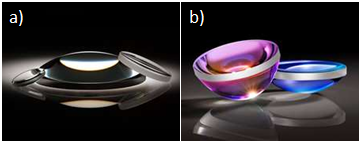
\includegraphics[width=8cm]{pictures/lenses.png}
\end{center}
\caption{a) Lentilles minces, b) Lentilles asphériques épaisses. Source : \textcopyright Edmund Optics }
\label{fig:lentille_mince}
\end{figure}

L'axe optique de la lentille est défini par la droite passant par les deux centres de courbure $C$ et $C'$ des deux dioptres. Par convention, on définit le sens positif comme le sens de propagation de la lumière.  La distance focale $f$ d'une lentille dans l'air est donnée par la "formule des opticiens" Eq.~\ref{eq:lensmaker} où $n$ est l'indice du matériau à la longueur d'onde de travail, et $R_{1, 2}$ respectivement rayons de courbure des dioptres arrière et avant de la lentille. 
\begin{equation}
\label{eq:lensmaker}
\frac{1}{f}=(n-1)\left[\frac{1}{R_1}-\frac{1}{R_2}+\frac{(n-1)d}{n R_1 R_2}\right]
\end{equation}
Tout système optique possède deux foyers, un foyer objet et un foyer image. Pour une lentille mince, ces foyers sont sur l'axe optique et symétriques par rapport au centre $O$ de la lentille. Le demi-espace délimité par le plan contenant la lentille porte le nom du foyer qu'il contient (espace objet ou espace image). Un objet réel se situe dans l'espace objet et un objet virtuel dans l'espace image, il en va de même pour une image, qui sera réelle si elle se situe dans l'espace image et virtuelle si elle se trouve dans l'espace objet.


\subsection{Formule(s) de conjugaison et construction d'images}

La formule de conjugaison est la relation entre la focale de la lentille et les positions de l'objet et de l'image. La formule dite "de Descartes" s'écrit~:
\begin{equation}
\label{eq:descartes}
\frac{1}{\overline{OF}}=\frac{1}{\overline{OA'}}-\frac{1}{\overline{OA}}
\end{equation}
On peut en déduire la formule de Newton pour un système optique centré : 
\begin{equation}
\label{eq:newton}
\overline{FA}\cdot\overline{F'A'}=-\overline{OF'}^2
\end{equation}

\begin{figure}[!htbp]
\label{fig:image_lentille_convergente}
\begin{center}
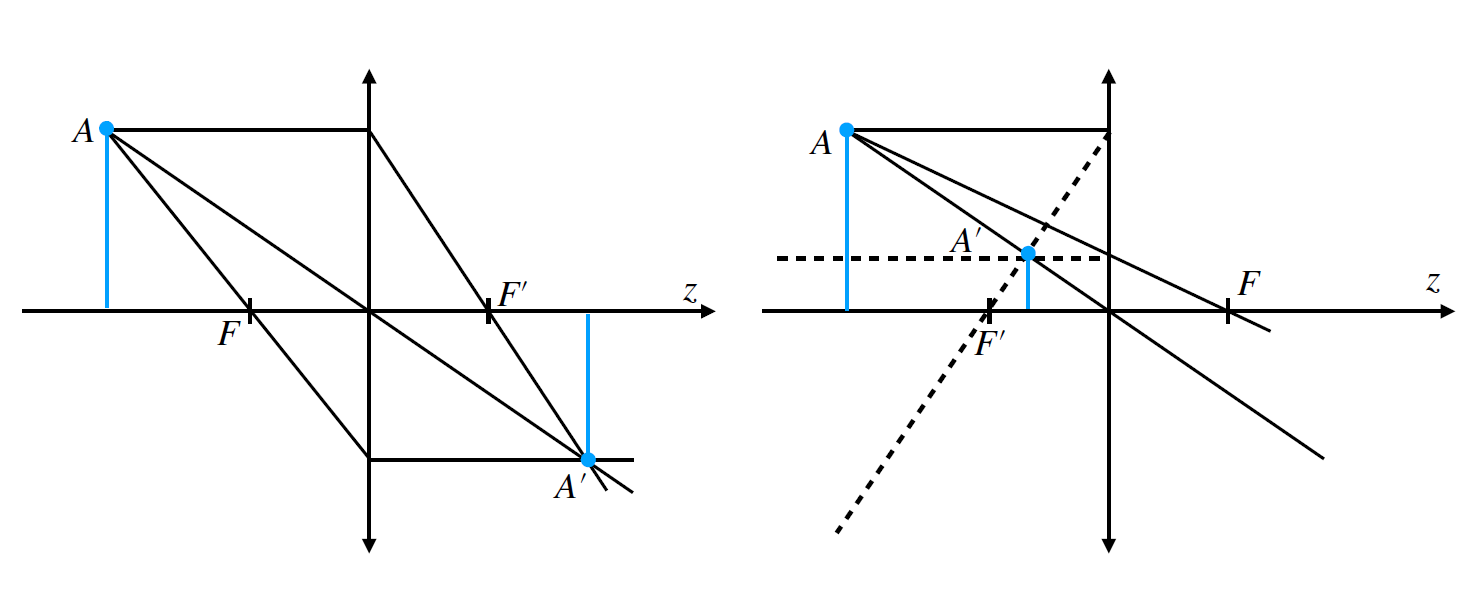
\includegraphics[width=15cm]{pictures/imageConstruction.png}
\end{center}
\caption{Construction d'une image par des lentilles}
\end{figure}

Afin de construire l'image d'un objet par une lentille, on se souviendra des règles suivantes : 
\begin{itemize}
    \item Un rayon passant par le centre optique n'est pas dévié
    \item Un rayon parallèle à l'axe optique focalise au foyer image
\end{itemize}
On remarquera que par retour inverse de la lumière, un faisceau sortant d'une optique parallèlement à l'axe provient du foyer objet.


Une quantité utile (ne serait-ce que pour choisir le bon objectif pour son appareil photo) est le grandissement du système. On le note $g$ et il est défini par~:
\begin{equation}
\label{eq:grandissement}
g=\frac{\overline{A'B'}}{\overline{AB}}=\frac{\overline{OA'}}{\overline{OA}}
\end{equation}

\subsection{Application aux miroirs sphériques}

Comme nous le verrons d'ici quelques cours, la construction de lasers implique l'utilisation intensive de miroirs courbes. La construction d'images par ces systèmes optiques est très similaire à la construction d'images par une lentille à ceci près qu'un miroir inverse évidemment le sens de propagation de la la lumière. Souvenez-vous que par convention, le sens positif est le sens de propagation de la lumière, il faut donc rédéfinir ce sens après chaque réflexion ! 

Un miroir concave est convergent, un miroir convexe est divergent. La focale d'un miroir sphérique est égale à la moitié de son rayon de courbure en mesure algébrique : $\overline{SF}=\frac{\overline{SC}}{2}$. $S$ est le sommêt du miroir (\textit{n'importe quel point de la surface est un sommet ! Par convention, on appelle S le point de la surface situé sur l'axe optique du miroir}) et $C$ son centre de courbure.
\textit{Petit exercice : montrer géométriquement qu'un miroir sphérique n'est pas parfaitement stigmatique}


\begin{figure}[!htbp]
\label{fig:miroir_concave}
\begin{center}
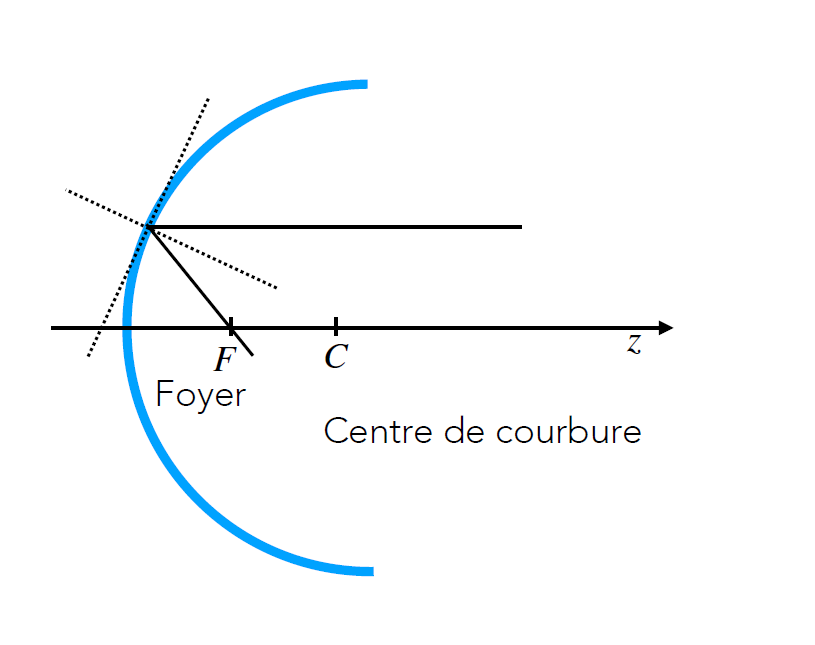
\includegraphics[width=8cm]{pictures/SpherMirr.png}
\end{center}
\caption{Tracé de rayons lumineux pour un miroir concave}
\end{figure}

Du fait de l'inversion du sens de propagation de la lumière après réflexion, la formule de conjugaison "de Descartes" pour un miroir sphérique est alors~: $\frac{2}{\overline{SC}}=\frac{1}{\overline{SA'}}+\frac{1}{\overline{SA}}$, et le grandissement $g = \frac{\overline{FS}}{\overline{FA}}$

\subsection{Petite digression sur les aberrations}

On peut facilement montrer que les rayons fortment hors-axe ne sont pas focalisés au même point que les rayons paraxiaux par une optique sphérique. Cette propriété géométrique est ce qu'on appelle une aberration géométrique. Il y en a beaucoup d'autres (dont l'astigmatisme -pouvant affecter les yeux- donnant lieu à l'existence de deux foyers distincts pour deux directions orthogonales perpendiculaires à l'axe optique). La seule surface permettant une focalisation parfaitement stigmatique quel que soit l'écart à l'axe optique d'un rayon parallèle à ce dernier est la parabole (c'est de ça dont il s'agit quand on parle d'optiques asphérisées, comme les lentilles des téléphones portables ou les lentilles de collimation des diodes laser).

\begin{figure}
    \centering
    \begin{minipage}{0.6\textwidth}
        \centering
        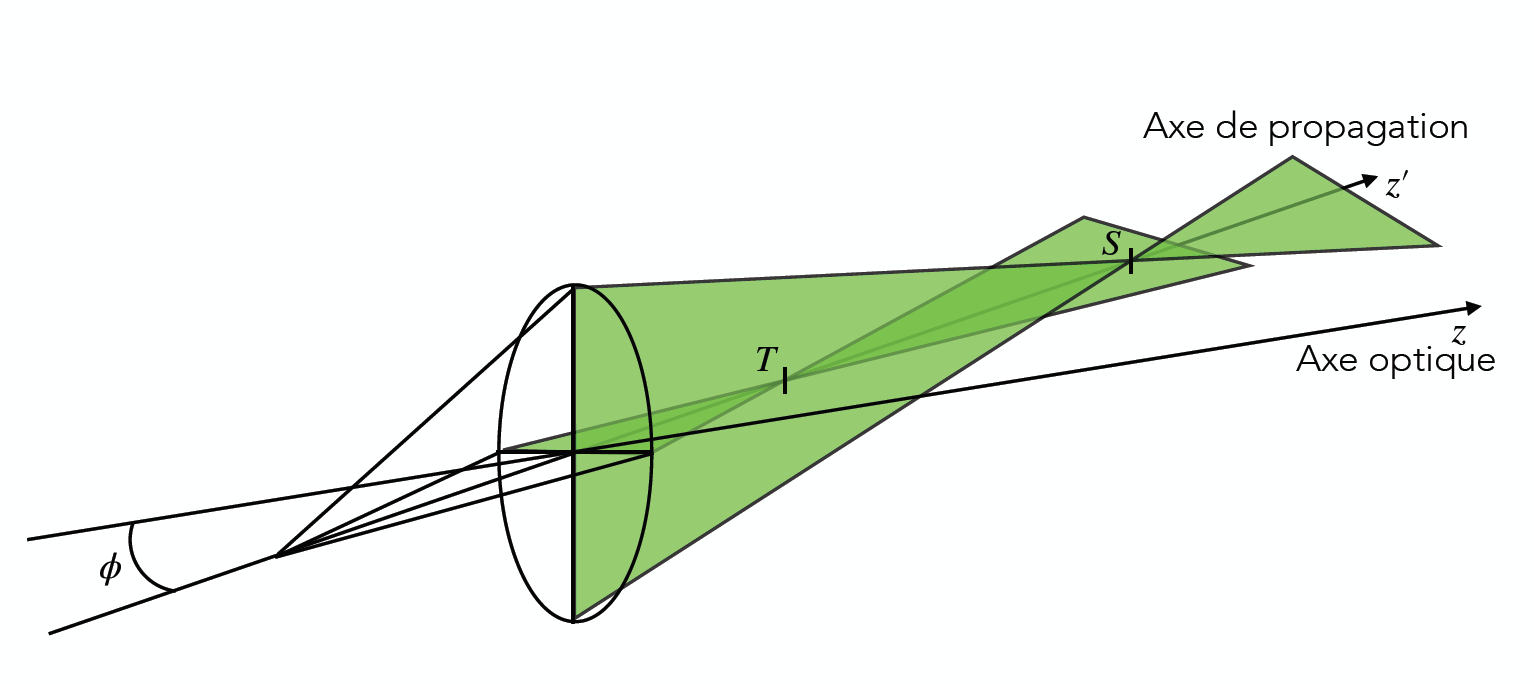
\includegraphics[width=1.\textwidth]{pictures/Astig.png} % first figure itself
        \caption{Astigmatisme}
    \end{minipage}\hfill
    \begin{minipage}{0.4\textwidth}
        \centering
        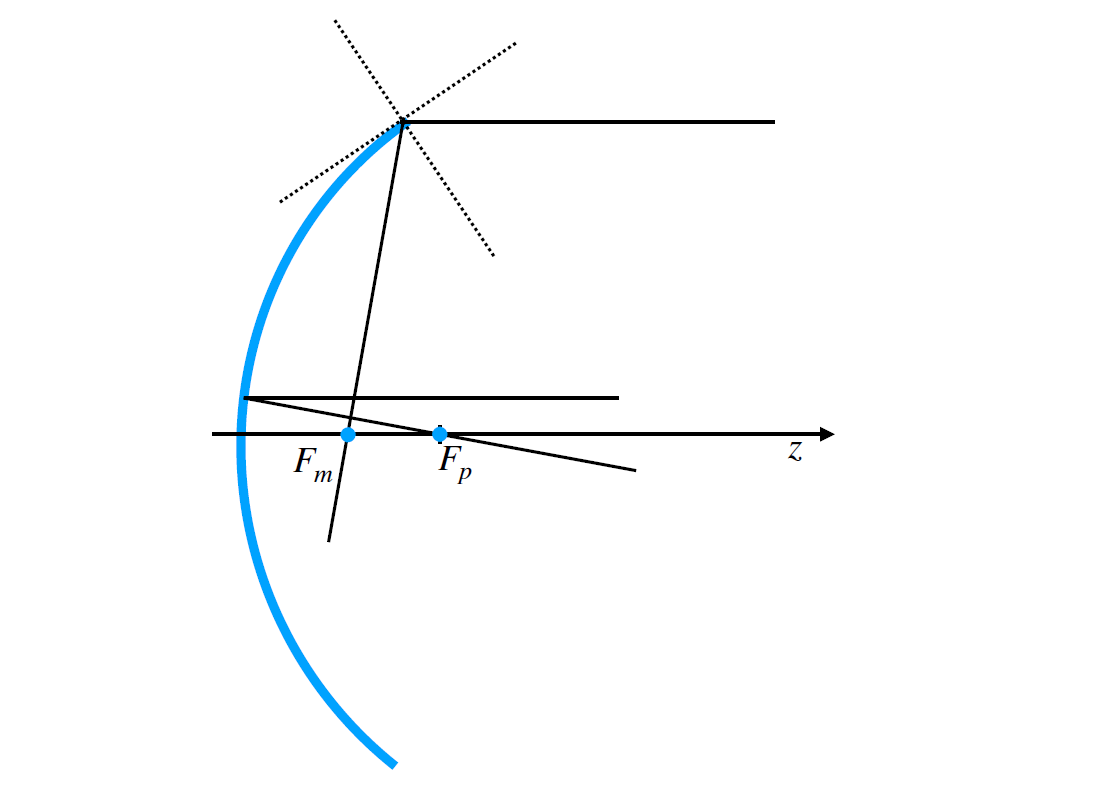
\includegraphics[width=1.0\textwidth]{pictures/abSpher.png} % second figure itself
        \caption{Aberration sphérique}
    \end{minipage}
\end{figure}


On remarque aussi que la formule dite "des opticiens" \ref{eq:lensmaker} dépend de l'indice de réfraction qui est une fonction de la longueur d'onde (voir par exemple https://refractiveindex.info/). Cela implique que la focale dépend de la longueur d'onde, donnant lieu à ce qu'on appelle l'aberration chromatique. Afin d'y remédier, on peut souvent utiliser des miroirs (achromatiques dans le sens des aberrations) ou des optiques spéciales combinant plusieurs verres pour compenser la variation d'indice avec la longueur d'onde. C'est le cas notamment des objectifs d'appareil photo, conçus pour travailler dans tout le spectre visible, ou d'un grand nombre d'objectifs de microscope. 

\section{Description matricielle d'éléments optiques}

Un ensemble de systèmes optiques travaillant dans les conditions de Gauss (== optique paraxiale) constitue une application linéaire, on peut donc exprimer les trajectoires des rayons par produits de \textit{matrices de transfert}, aussi appelées matrices de Gauss. Ce formalisme est  très pratique pour calculer numériquement la propagation d'un grand ensemble de rayons, notamment lors de la conception de cavités laser (voir section suivante!).

Un rayon est complètement caractérisé dans un plan orthogonal à l'axe par sa distance $r$ à l'axe optique et l'angle définissant sa direction de propagation $\theta$. La convention de signe pour les angles est la même qu'en trigonométrie : angles positifs dans le sens inverse des aiguilles d'une montre et zéro au niveau de l'axe optique. 
L'approximation paraxiale nous permettra d'assimiler $\mathrm{sin}(\theta)\sim\mathrm{tan}(\theta)\sim\theta$, et on aura une relation linéraire entre $\left(r_1, \theta_1\right)$ et $\left(r_2, \theta_2\right)$, positions et angles avant et après passage dans le système optique. Si on définit $r_1'$ et $r_1$ tels que $\theta_1 \sim (dr/dz)_z_1 = r_1'$ et $\theta_2 \sim (dr/dz)_z_2 = r_2'$, on peut alors écrire~: 

\begin{align} 
r_2 &=  Ar_1 + Br'_1 \\ 
r_2' &=  Cr_1 + Dr'_1
\end{align}
où $A, B, C, D$ sont des constantes caractéristiques de l'élément optique. Dans une formulation matricielle, on écrira naturellement~:

\begin{gather}
 \begin{bmatrix} r_2 \\ r'_2 \end{bmatrix}
 =
  \begin{bmatrix}
   A & B \\
   C & D 
   \end{bmatrix}
   \begin{bmatrix} r1 \\ r'_1 \end{bmatrix}
\end{gather}

\begin{figure}[!htbp]
\begin{center}
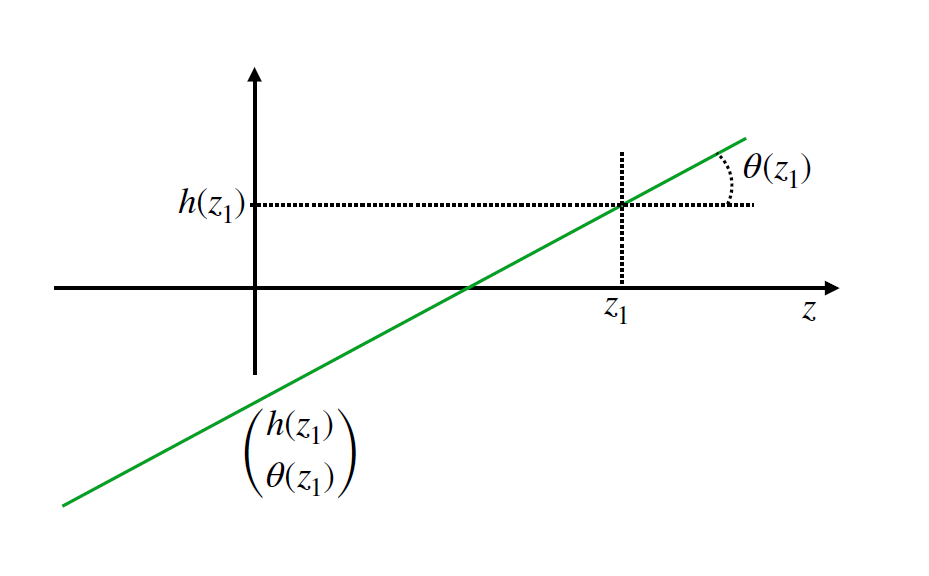
\includegraphics[width=10cm]{pictures/ABCD.png}
\end{center}
\caption{Schéma de principe de la représentation en matrices de transfert}
\label{fig:matrix}
\end{figure}


\subsection{\'Elements de base}\label{subsec:el_base}

\subsubsection{Propagation libre sur une distance L}
L'exemple le plus simple que nous pouvons prendre est celui de la propagation libre d'un rayon dans l'air sur une distance $L$. A titre d'exercice, on évaluera aussi la propagation d'un rayon dans un milieu d'indice $n$ pour des plans d'entrée et de sortie juste à l'extérieur de ce milieu.
\subsubsection{Traversée d'un dioptre plan}
\subsubsection{Traversée d'une lentille mince de focale $f$}
\subsubsection{Traversée d'un dioptre sphérique de rayon $R$}
\subsubsection{Matrice de transfert entre deux plans conjugés}
\textit{Pour vous amuser...}

Pour tous les exemples donnés ci-dessus, on notera que le déterminant de la matrice $ABCD$ est égal au rapport des indices de réfraction d'entrée et de sortie : $AD - BC = \frac{n_1}{n_2}$. Dans la plupart des cas concrets, les milieux d'entrée et de sortie sont les mêmes, par conséquent, le déterminant de la matrice $ABCD$ sera égal à 1.

\section{Application des matrices de transfert aux cavités}
Une des applications du formalisme des matrices de transfert est l'étude de la stabilité des cavités. Nous allons voir dans cette partie comment l'utiliser.

\subsection{Condition de stabilité}

Nous nous intéressons ici à la propagation des rayons lumineux dans une une cavité dans laquelle on se fixe un plan $\Pi$ de référence, et dont on connaît la matrice de transfert $T$ sur un tour (le départ du plan $\Pi$ et retour au plan $\Pi$ après traversée de toutes les optiques de la cavité forme ce que l'on appelle une cellule unitaire de la cavité, comme indiqué sur la figure~\ref{fig:cell}). 


\begin{figure}[!htbp]
\begin{center}
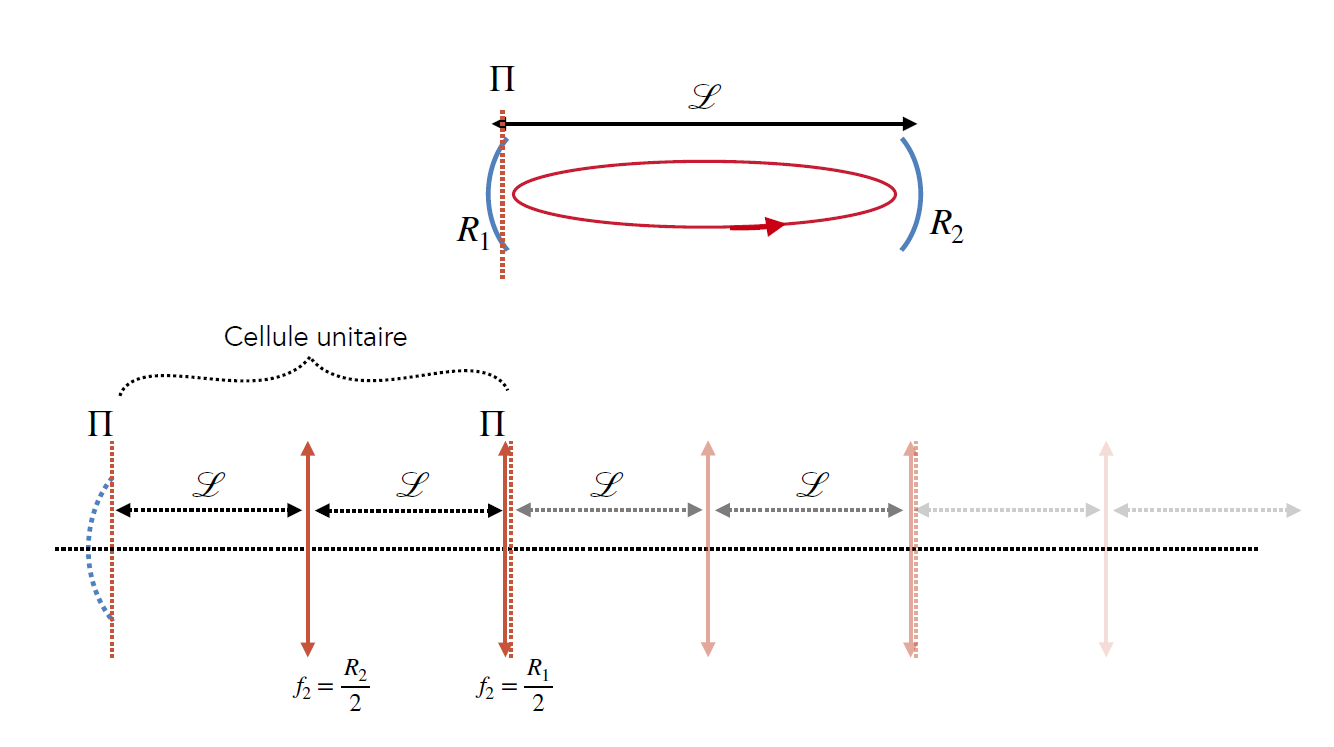
\includegraphics[width=15cm]{pictures/cell.png}
\end{center}
\caption{Cavité linéaire déployée en cellules unitaires consécutives, exemple pour une cavité linéaire}
\label{fig:cell}
\end{figure}

Après $n$ tours de cavité, un rayon de coordonnées $\left[r, r'\right]$ dans le plan $\Pi$ peut soit rester au voisinage de l'axe soit s'en éloigner. Une cavité pour laquelle les rayons restent confinés est dite stable. Lorsque les rayons divergent en-dehors de la cavité, cette cavité est instable. 
\textbf{Nous cherchons ici à établir une relation générale nous permettant d'évaluer si la cavité est stable ou pas.}  

Dans le cas général, les coordonnées $\left[r_n, r'_n\right]$ sont exprimées par~:
\begin{gather}
 \begin{bmatrix} r_n \\ r'_n \end{bmatrix}
 =
\left[T\right]^n
   \begin{bmatrix} r \\ r' \end{bmatrix}
\end{gather}

Si le résonateur est stable, pour tout rayon initial de coordonnées $\left[r_0, r'_0\right]$, le rayon $\left[r_n, r'_n\right]$ ne doit pas diverger lorsque $n$ augmente. Cela implique que~:
\begin{gather}
  \begin{bmatrix}
   A & B \\
   C & D 
   \end{bmatrix}^n
\end{gather}
ne diverge pas.

Lorsqu'un rayon effectue un tour complet de cavité, l'indice d'entrée et l'indice de sortie sont évidemment identiques, le déterminant de la matrice de transfert $T$ de la cavité $AD-BC$ est par conséquent égal  1. Grâce au théorème de Sylvestre \cite{bornwolf}, et en posant $\mathrm{cos}(\theta) = (A+D)/2$, on peut montrer que~:
\begin{gather}
  \begin{bmatrix}
   A & B \\
   C & D 
   \end{bmatrix}^n
 =\frac{1}{\mathrm{sin}(\theta)}
   \begin{bmatrix}
   A \mathrm{sin}(n\theta) - \sin\left((n-1)\theta\right) & B\sin (n\theta) \\
   C\sin (n\theta) & D\sin (n\theta) - \sin\left((n-1)\theta \right)
   \end{bmatrix}
\end{gather}
Cette relation montre que la n-ième puissance de la matrice $T$ ne diverge pas si $\theta$ est réel. En effet, si on écrit~:

\begin{equation}
\label{eq:thetaib}
    \theta = a + ib
\end{equation}

alors : 
\begin{align*}
     \sin (n\theta) &= \left[\exp(in\theta)+\exp(-in\theta)\right]/2i \\
     &=\left[\exp(ina - nb)+\exp(-ina + nb)\right]/2i 
\end{align*}

La quantité $\sin n\theta$ contiendrait donc un terme \textit{exponentiellement croissant} avec $n$ pour $|b|>0$, la matrice $T^n$ divergerait alors. Par conséquent, pour que le résonanteur soit stable, $\theta$ doit être réel, et d'après l'équation \ref{eq:thetaib}, cela implique~:

\begin{equation}
\label{eq:stab}
 -1<\left(\frac{A+D}{2}\right)<1
\end{equation}

Cette équation établit la condition de stabilité pour tout résonateur travaillant dans les conditions paraxiales. 


On peut aussi démontrer cette condition par diagonalisation de la matrice $T$. 
En utilisant le fait que le déterminant de la matrice vaille 1 sur un tour (milieux d'arrivée et de départ identique), la résolution de $\det\left[T-\lambda I\right] = 0$ amène à l'équation aux valeurs propres suivante~:
\begin{equation}
\lambda^2- \lambda \Tr{T}+1 = 0
\end{equation}
Cette équation admet deux solutions (que l'on peut écrire sous forme exponentielle) $\lambda_+ = \rho_+\exp^{i\phi_+}$ et  $\lambda_- = \rho_-\exp^{i\phi_-}$~: 

\begin{equation}
\label{eq:eigenval}
    \lambda_\pm=
    \frac{\Tr{T}}{2}
    \pm
    \sqrt{
    \left(
    \frac{\Tr{T}}
    {2}
    \right)^2-1
    }
\end{equation}
On rappelle que  $\det{T}=\lambda_{+}\lambda_{-} = 1$, par conséquent, si $\lambda_+ = \rho_+\exp^{i\phi_+}$ alors $\lambda_- = \rho_+^{-1}\exp^{-i\phi_+}$. 

Lorsque $\lambda_{+}$ et $\lambda_{-}$ sont distinctes, les vecteurs propres associés $u_{+},\,u_{-}$ forment une base, et on peut alors exprimer tout rayon $x = \left[r_n, r'_n\right]$ comme une combinaison linéaire de ces deux vecteurs propres $x = au_{+}+bu_{-}$. 

Après $n$ tours de cavité, $x_n = a(\lambda_+)^nu_{+}+b(\lambda_-)^nu_{-}$. Ce rayon reste borné si $|\lambda_+|\leq1$ et $|\lambda_-|\leq1$. Comme $\lambda_{+}\lambda_{-} = 1$, alors $|\lambda_+|=|\lambda_-|=1$. 
Puisque $\Tr{T}=\lambda_+ + \lambda_-=A+D$, on obtient~:
\begin{equation}
    2\cos\phi = A + D
\end{equation}
Nous retrouvons alors la condition de stabilité~:

\begin{equation}
    -1\leq \frac{A+D}{2}\leq 1
\end{equation}
ou encore :
\begin{equation}
    0 \leq \frac{A+D+2}{4}\leq 1
\end{equation}

\subsection{Exemple pour une cavité linéraire}\label{subsec:ex_cavlin}


Maintenant que nous avons établi une relation générale permettant d'évaluer si la cavité que l'on cherche à concevoir sera stable ou pas, nous pouvons étudier le cas particulier d'une cavité linéaire.


La matrice $ABCD$ associée à la cavité de la Figure~\ref{fig:cell} est obtenue par le produit ordonné des matrices des éléments optiques individuels qui la constituent. \\



En reprenant les éléments de base dérivés page~\pageref{subsec:el_base}, on construit ainsi~:

\begin{gather}
  \begin{bmatrix}
   A & B \\
   C & D 
   \end{bmatrix}
   =
  \begin{bmatrix}
   1 & 0 \\
   -2/R_1 & 1 
  \end{bmatrix}
  \begin{bmatrix}
   1 & L \\
   0 & 1 
   \end{bmatrix}
  \begin{bmatrix}
   1 & 0 \\
   -2/R_2 & 1 
  \end{bmatrix}
  \begin{bmatrix}
   1 & L \\
   0 & 1 
   \end{bmatrix}
\end{gather}

D'où on calcule~:
\begin{align}
\label{eq:stab_cav_lin}
    \frac{A+D}{2}&=1-\frac{2L}{R_1}-\frac{2L}{R_2}+\frac{2L^2}{R_1R_2}\\
                 &=2\left[1-\frac{L}{R_1}\right]\left[1-\frac{L}{R_2}\right]-1
\end{align}

Il est commun de définir les paramètres $g_1 = 1 -\left(\frac{L}{R_1}\right)$ et $g_2 = 1 -\left(\frac{L}{R_2}\right)$, qui nous permettent de réécrire l'équation~\ref{eq:stab_cav_lin} de façon très simple~:

\begin{equation}
    0<g_1g_2<1
\end{equation}

Nous pouvons alors tracer le diagramme de stabilité général pour un résonateur sphérique (Figure~\ref{fig:diag_stab}). 

\begin{figure}[!htbp]
\begin{center}
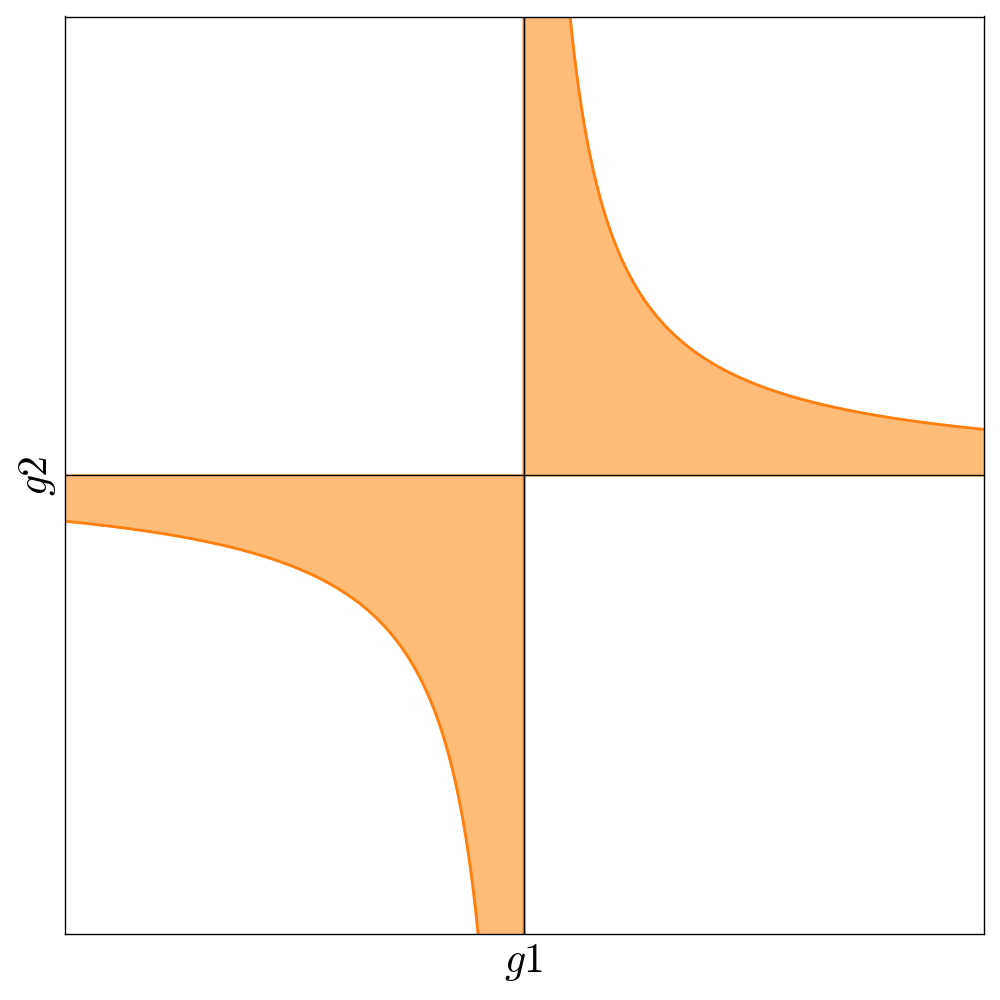
\includegraphics[width=12cm]{pictures/stability.png}
\end{center}
\caption{Diagramme de stabilité : sur ce diagramme, situez la cavité confocale, la cavité concentrique et le Fabry-Pérot plan-plan. Où se situent les cavités symétriques ? (Schéma à compléter à la main par vos soins !)}
\label{fig:diag_stab}
\end{figure}

\subsection{Pour aller plus loin...}
https://doi.org/10.1364/OL.27.001869

\chapter{Faisceaux Gaussiens}

Bien que l'approche géométrique permette d'aller aussi loin que l'évaluation de la stabilité des cavités, elle est évidemment insuffisante à une analyse complète de la lumière en cavité puisque les effets d'interférence et de diffraction ne sont pas décrits. Lors du cours XXX il a été démontré que dans l'approximation paraxiale, le champ électrique scalaire en un point $r(x, y, z)$ éloigné de la source $r_0(x_0, y_0, z_0)$ peut s'écrire~: 

\begin{equation}
    E(r,r_0) \propto \frac{1}{z-z_0}\mathrm{e}^{-ik(z-z_0)}\exp\left[-\iu k\frac{(r - r_0)^2}{2(z - z_0)}\right]
    \label{eq:chp_gaussien}
\end{equation}

%Soit $R_0$ le rayon de courbure de l'onde au point $z_0$, alors le rayon de l'onde au point $z$ est donné par :
%\begin{equation}
%    R(z) = R_0+z-z_0
%\end{equation}

Il s'agit du champ d'une onde paraxiale, qui est une solution approchée de l'équation de Helmholtz où l'on reconnaît le facteur de propagation $\exp(-ik(z-z_0))$ et le facteur de variation transverse d'amplitude~:

\begin{equation}
    u(x, y, z) = \frac{1}{z-z_0}\exp\left[-ik\frac{(x-x_0)^2+(y-y_0)^2}{2(z-z_0)}\right]
\end{equation}

Nous allons à présent transformer l'expression du champ éléctrique \ref{eq:chp_gaussien} afin d'en donner une interprétation physique. 

On introduit le rayon de courbure complexe~: 
\begin{equation}
    q(z)=q_0+z_{z_{0}}
\end{equation}

puis on réécrit la répartition transverse d'amplitude sous la forme~: 

\begin{equation}
    u(x, y, z) = \frac{1}{q(z)}\exp\left(-ik\frac{x^2+y^2}{2q(z)}\right)
\end{equation}

En séparant les parties réelle et imaginaire de $q(z)$ telles que $\frac{1}{q(z)}=\frac{1}{R(z)}-\frac{\iu}{q_i(z)}$, on obtient~:

\begin{equation}
    u(x,y,z)=\frac{1}{q(z)}\exp\left(-\iu k \frac{x^2 + y^2}{2q_r(z)}\right)\exp\left(-\iu k \frac{x^2 + y^2}{2q_i(z)}\right)
\end{equation}

où nous avons ainsi fait apparaître un terme de phase quadratique dont le rayon de courbure est égal à $q_r(z)$ et un profil d'amplitude gaussien de demi-largeur à $1/e^2$ égal à $q_i(z)$. Par souci de lisibilité, on adopte la notation suivante~:

\begin{equation}
    q_r(z)=R(z)\quad\mathrm{et}\quad w^2(z)=\frac{k}{2q_i(z)}
\end{equation}

$R(z)$ correspondant à un rayon de courbure et $w(z)$ au ``waist'' en anglais ou col en français, pour une abscisse $z$. Attention, $R(z)$ ne peut plus être déduit d'un rayon de courbure précédent par simple relation linéaire, comme en optique paraxiale. On remarque de plus que physiquement, $q_i(z)$ ne peut être que positif puisque par conservation de l'énergie, l'amplitude d'un champ dont l'étendue spatiale augmente ne peut pas croître. 
On obtient ainsi deux relations qui nous seront très utiles :

\begin{align}
    \frac{1}{q(z)}&=\frac{1}{R(z)}-\frac{\iu \lambda}{\pi w^2(z)}\\
    u(x,y,z)&=\frac{1}{q(z)}\exp\left(-\iu k \frac{x^2 + y^2}{2R(z)}\right)\exp\left(-\frac{x^2 + y^2}{w^2(z)}\right)
\end{align}
    


\section{Propagation libre de l'onde Gaussienne}

On cherche ici à connaître l'évolution des paramètres w et R après propagation libre sur une distance $z-z_0$, en supposant ces paramètres connus dans un plan transverse donné. $z-z_0$ étant réel, il existe nécessairement un plan $\Pi_0$ de l'axe de propagation pour lequel $q$ est un imaginaire pur que l'on notera $q_0$. D'après la définition de $q$, sur ce plan particulier, la surface d'onde est infinie (onde plane) et on a~:

\begin{equation}
    R_0 = \infty \quad \textrm{et} \quad q_0=i\frac{\pi w_0^2}{\lambda} = iz_R
\end{equation}

$z_R$ est une distance caractéristique que l'on appelle la longueur de Rayleigh. Ce paramètre est important et reviendra régulièrement dans les chapitres à venir.
Par la suite, on prendra la position du plan $\Pi_0$ pour origine sur l'axe de propagation ($z_0=0$).

A partir de ce plan, on a donc :
\begin{align}
    q(z) &= q_0+z\\
    \frac{1}{q(z)}&=\frac{1}{z+iz_R}\\
    \textrm{et} \quad \frac{1}{q(z)}&=\frac{1}{R(z)}-i\frac{\lambda}{\pi w^2(z)}
\end{align}
De ces équations, on tire les relations donnant l'évolution de $R$ et $w$ en fonction de la distance parcourue $z$~:

\begin{align}
  R(z) &= z + \frac{z_R^2}{z}\\
  w^2(z)&= w_0^2\left[1+\left(\frac{z}{z_R}\right)^2\right]  = \frac{\lambda}{\pi}\left(z_R+\frac{z^2}{z_R}\right)
\end{align}

De ces équations, on tire que :
\begin{itemize}
    \item Sur le plan $\Pi_0$, la taille du faisceau gaussien est minimale et son rayon transverse vaut $w_0$. Ce lieu particulier est appelé waist du faisceau ou encore  ``col" en français
    \item Le faisceau est symétrique par rapport au plan du waist
    \item Le rayon transverse $w(z$) varie de manière hyperbolique suivant $z$.
\end{itemize}

Quand $z\gg Z_R$, alors $w(z)\simeq\frac{w_0z}{z_R}\simeq \theta z$ où $\theta = \frac{\lambda}{\pi w_0}$ est le demi-angle de divergence à $1/$e de
l'amplitude. $\theta$ est l'angle formé par les asymptotes à l'hyperbole à grande
distance du plan $\Pi_0$ (cf. Fig.~\ref{fig:carac_gauss}).
La longueur de Rayleigh permet de définir deux régimes de propagation :
\begin{itemize}
    \item $z_R < z < z_R$ : les lois de l'optique géométrique classique ne sont pas valables.
    \item $|z|\gg z_R$ : il est possible d'utiliser l'optique géométrique.
\end{itemize}


\begin{figure}[!htbp]
\begin{center}
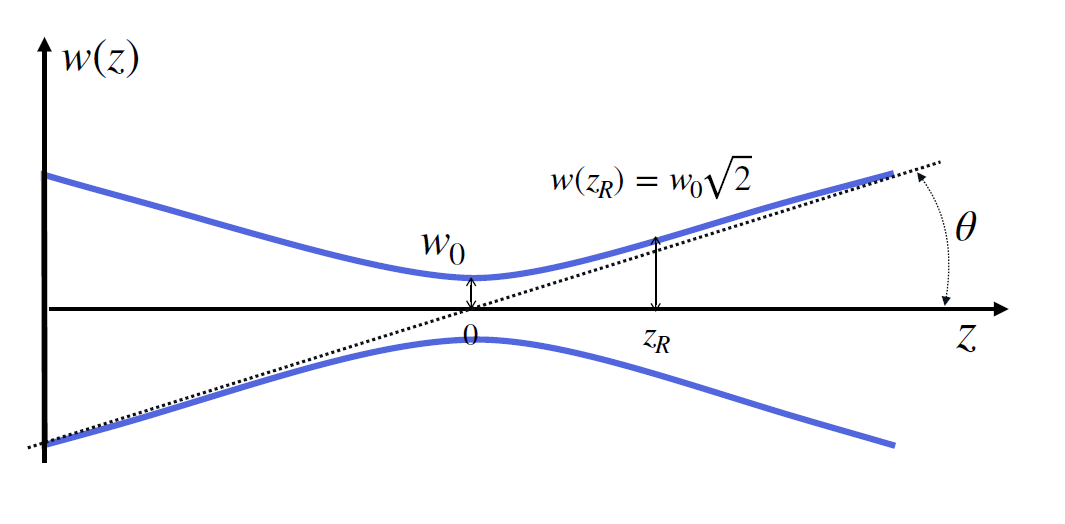
\includegraphics[width=10cm]{pictures/gaussian.png}
\end{center}
\caption{Caractéristiques du faisceau gaussien}
\label{fig:carac_gauss}
\end{figure}

Le rayon de courbure de l'onde est plan en $z=0$, il est minimum en $z = z_R$ ($R_\textrm{min}=2z_R$) et il vaut environ $z$ quand $z$ est grand devant la longueur de Rayleigh.


\section{Faisceaux Gaussiens et matrices ABCD}

Il est possible de démontrer dans le cas général (ce que nous ne ferons pas ici), qu'après traversée d'un système optique décrit par une matrice $ABCD$, une onde gaussienne de rayon de courbure complexe $q$ se transforme en une autre onde gaussienne de rayon de courbure complexe $q'$ donné par~:

\begin{equation}
    q'=\frac{Aq+B}{Cq+D}
\end{equation}
C'est ce qu'on appelle \textit{la loi ABCD}.

\subsection{Formules de conjugaison d'un faisceau gaussien}

En utilisant la loi ABCD appliquée à un système optique centré avec origines aux foyers, on peut trouver les relations entre les positions et les tailles d'un waist objet situé avant le système optique et celles du waist image obtenu après traversée du système.


Le waist objet $w_0$ est situé sur le plan repéré par l'abscisse $\sigma$ par rapport au foyer objet tandis que le waist image $w'_0$ est repéré par l'abscisse $\sigma'$ par rapport au foyer image (cf. Figure~\ref{fig:conjugaison_gauss}). Le rayon de courbure complexe correspondant au waist objet est imaginaire pur et vaut :

\begin{equation}
    q_0=\iu \frac{\pi w_0^2}{\lambda}
\end{equation}

Les éléments de la matrice de transfert valent (démonstration en TD):
\begin{equation}
    A=\frac{-\sigma'}{f'};\,B=-f+\frac{\sigma \sigma'}{f'};\,C=-\frac{1}{f'};\,D=\frac{\sigma}{f'}
\end{equation}

En appliquant la loi ABCD et sachant que $q_0$ et $q_0'$ sont tous les deux des imaginaires purs, on trouve les relations suivantes :

\begin{align}
    \sigma \sigma'&=ff'-q_0q_0'\\
    \sigma q_0 &= \sigma'q_0\\
    \sigma \sigma' &= ff' + z_RzR'\\
    -\frac{\sigma}{z_R}&=\frac{\sigma'}{z_R}
\end{align}

Ces relations démontrent que la position du waist image dépend non seulement de la position du waist objet mais aussi de sa taille. Lorsque $\sigma>>z_R$, l'onde au niveau du foyer objet est quasi-sphérique (celui-ci est dans le champ lointain du faisceau). Le front d'onde au niveau de la lentille s'apparente donc semble donc au front d'onde d'un point source, et on obtient alors : $\sigma\sigma'=ff'$. On retrouve ici les relations de Newton de l'optique géométrique.
Un autre cas particulier est le cas $\sigma=0$. Dans ce cas, on a aussi $\sigma'=0$. Le waist image est situé exactement sur le foyer image et la relation de grandissement entre les waists est donnée par~:

\begin{equation}
    w_0'^2=-\frac{1}{w_0^2}\frac{ff'\lambda\lambda'}{\pi^2}
\end{equation}

\begin{figure}[!htbp]
\begin{center}
\includegraphics[width=8cm]{}
\end{center}
\caption{Abscisses des waists objet et image}
\label{fig:conjugaison_gauss}
\end{figure}


\subsection{Déphasage d'un faisceau gaussien par propagation}

Le déphasage sur l'axe Oz par propagation du faisceau entre les plans de référence est donné par~:
\begin{equation}
    \phi(z) = -kz-\arg(A+B/q) = \phi_0+\phi_g
\end{equation}

Le terme $\phi_0$ représente le déphasage par propagation d'une onde plane et le terme $\phi_g$ est la phase de Gouy. En prenant pour origine le waist du faisceau, on peut calculer le terme $\phi_g$ correspondant à une propagation libre~:
\begin{equation}
    A+\frac{B}{q}=1+\frac{z}{\iu z_R}
\end{equation}

d'où on déduit~:
\begin{equation}
    \phi(z) = -kz-\arctan\left(\frac{z}{z_R}\right)
\end{equation}

Lorsque $w_0$ ou $Z_R$ deviennent très grands, le faisceau gaussien devient proche d'une onde plane et on voit alors que le déphasage $\phi_g$ tend vers zéro.



\medskip

\noindent\fcolorbox{black}{myGray}{%
    \minipage[t]{\dimexpr1\linewidth-2\fboxsep-2\fboxrule\relax}
        \textbf{Calculs de la taille et de la position du waist en cavité :\\}
            Soit une cavité linéaire de longueur $L$ et dont les miroirs sont de courbures $R_1$ et $R_2$
          \\
          \\
          \begin{itemize}
              \item  Etablir le système de trois équations sur les trois inconnues $z_1, z_2$ et $z_R^2$
              \\\\\\
              \item  En utilisant la relation $L = z_2 - z_1$, résoudre ce système et en déduire la position et la taille du waist (attention, ne vous embarquez pas dans unr résolution de polynômes du 2e degré... Horrible !)
              \\\\\\
              \item  On introduit les paramètres $g_1 = 1-\frac{L}{R_1}$ et $g_2 = 1-\frac{L}{R_2}$. Retrouver la condition de stabilité de la cavité linéaire. 
              \\\\\\
          \end{itemize}
         
          \\\\
    \endminipage}\hfill
    
\medskip


\chapter{Résonateurs passifs}

Lors de ce chapitre, nous allons nous intéresser aux propriétés, notamment spectrales, des champs électriques résonants au sein de cavités \textit{passives}, c'est-à-dire en l'absence de milieu à gain. 
Les résonateurs utilisés dans les lasers sont composés de miroirs plans ou sphériques, et la longueur de la cavité va généralement de quelques centimètres à quelques dizaines de centimètres. 
Ces résonateurs sont dits ouverts, à la différence des résonateurs micro-ondes qui sont fermés et confinent ainsi le champ dans les trois dimensions. Les résonateurs ouverts en revanche présentent des pertes transverses du fait de la diffraction du champ. Cependant, il existe dans les résonateurs ouverts des modes comportant de très faibles pertes ; on définit un tel mode comme une configuration électromagnétique que l'on écrit~:

\begin{equation}
    E(r,t)=E_0u(r)\exp\left[(-t/2\tau_c)+\iu \omega t\right]
\end{equation}

La quantité $\tau_c$ est le temps de vie d'un photon en cavité.

\section{Fréquences de résonance}

\subsection{Cavité plan-plan (cavité Fabry-Pérot)}
Ce type de résonateur, que vous avez probablement étudié précédemment, est consrtuit par l'association de deux miroirs plans parallèles l'un à l'autre, et séparés par une distance $L$. En première approximation, on peut considérer que les modes de ce résonateur sont la superposition de deux ondes planes se propageant dans les deux directions opposées. On considèrera que les miroirs sont métalliques, et que par conséquent le champ au niveau du miroir s'annule. Par conséquent, on peut établir que la longueur de la cavité doit être un multiple de demi-entiers de la longeur d'onde $L = n(\lambda/2)$ où $n$ est un entier positif. On déduit ainsi la relation~:
\begin{equation}
    \nu = n\left(\frac{c}{2L}\right)
    \label{eq:FP}
\end{equation}
une relation que l'on peut aussi déduire en imposant que le déphasage de l'onde sur un aller-retour soit un multiple de $2\pi$, c'est-à-dire $2kL=2n\pi$ afin que l'interférence soit constructive et que le champ obtenu par une succession de réflexions soit non nul. 
On en tire aisément l'intervalle spectral libre : 
\begin{equation}
    \Delta\nu = \frac{c}{2L}
\end{equation}
qui est l'espacement fréquentiel entre deux modes \textit{longitudinaux} consécutifs.

\subsection{Cavité concentrique}
On construit un résonateur concentrique en plaçant deux miroirs sphériques de même rayon de courbure $R$ à une distance $L=2R$. Dans ce cas simple, les modes peuvent être approximés par une superposition de deux ondes sphériques prenant leur origine aux centres confondus des deux miroirs. On obtient ainsi la même relation de résonance que pour un résonateur Fabry-Pérot (Eq.~\ref{eq:FP}).

\begin{figure}[!htbp]
\begin{center}
\includegraphics[width=8cm]{}
\end{center}
\caption{Résonateur concentrique}
\label{fig:resonateur_concentrique}
\end{figure}

\subsection{Cavité confocale}
La combinaison de deux miroirs sphériques de rayons de courbure $R_1$ et $R_2$ à une distance telle que leurs \textbf{points focaux} soient confondus est un résonateur confocal. Dans le cas particulier de $R_1=R_2=R$, on a alors $L=R$. Comme le montre la figure~\ref{fig:resonateur_confocal}, on peut tracer un nombre infini de chemins optiques géométriques fermés dans ce type de cavité, et par conséquent on ne peut en déduire une relation simple avec les fréquences de résonance. 

\begin{figure}[!htbp]
\begin{center}
\includegraphics[width=8cm]{}
\end{center}
\caption{Résonateur confocal}
\label{fig:resonateur_confocal}
\end{figure}

\subsection{Cavité sphérique générale}
Dans le cas très général où les rayons de courbures et distances entre les miroirs sont arbitraires, on ne peut pas de façon générale trouver de rayon revenant à son point de départ, et de même que pour un résonateur confocal il est impossible par cette approche d'établir une condition de résonance. 

\subsection{Cavité en anneau}
Une cavité importante dans le domaine des lasers est la cavité en anneau qui peut être simple ou repliée. Elle peut être faite de miroirs plans et ou sphériques, comme indiqué Fig.~\ref{fig:ring_cavity}. Afin que l'onde revienne sur elle-même après un tour complet de cavité, on établit que~:

\begin{equation}
    \nu=\frac{nc}{L}
\end{equation}

\begin{figure}[!htbp]
\begin{center}
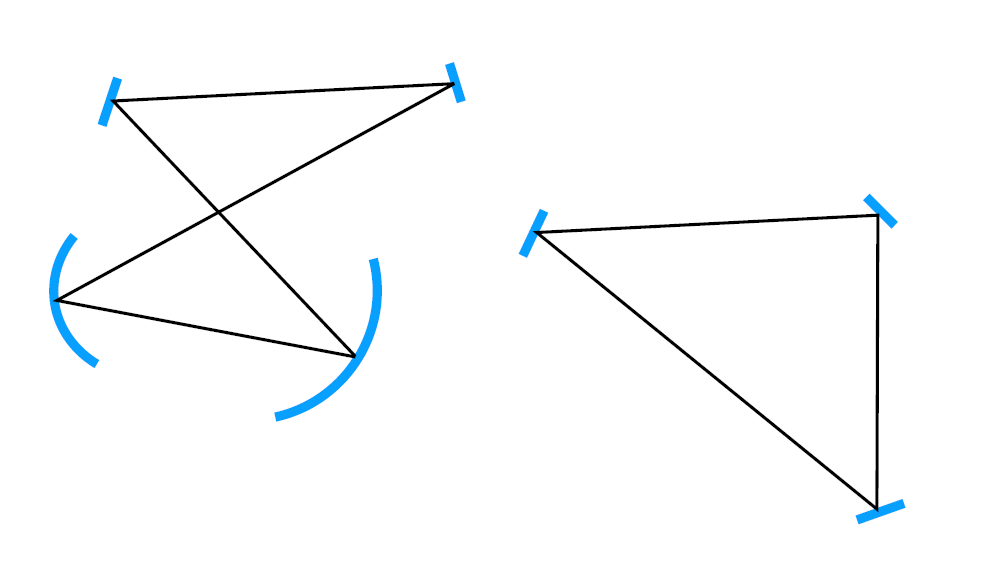
\includegraphics[width=8cm]{pictures/RingCav.png}
\end{center}
\caption{Cavités en anneau}
\label{fig:ring_cavity}
\end{figure}

\section{Modes propres, valeurs propres}


\begin{figure}[!htbp]
\begin{center}
\includegraphics[width=8cm]{}
\end{center}
\caption{Cavité à deux miroirs et structure linéaire équivalente}
\label{fig:eigenmodes_cavity}
\end{figure}

Jusqu'à présent, nous avons adopté une approche quasiment géométrique à l'établissement des conditions de résonance des \textbf{modes longitudinaux}. On peut dans le cas général dériver une telle condition si on prend en compte l'existence de \textbf{modes transverses}. 
Si on écrit l'amplitude du champ dans le cas décrit Fig.~\ref{fig:eigenmodes_cavity} après un tour complet de cavité \cite{svelto}, on obtient~:

\begin{equation}
    \tilde E(x,y,2L)=\left[\exp(-2\iu kL\right]\iint K(x,y; x_1,y_1)~E(x_1, y_1, 0)dx_1dy_1
    \label{eq:gen_field}
\end{equation}
$K(x,y; x_1,y_1)$ est ce que l'on appelle le noyau de propagation (voir encart ci-après). 
Afin que ce mode soit résonant, il faut que la forme du champ soit identique à elle-même après un tour complet de cavité. On établit donc que~: 

\begin{equation}
     \tilde E(x,y,2L)=\tilde\sigma\exp(-2\iu kL)\~E(x,y,0)
\end{equation}

$\sigma$ correspond à un facteur complexe constant donnant l'atténuation de l'onde par diffraction ainsi que son déphasage sur un tour complet. On réécrit $ \tilde\sigma = | \tilde\sigma|\exp(\iu \phi)$. On a alors deux contributions au terme de phase : longitudinale ($-2kL$) et une transverse ($\phi$). Le déphasage total est donc~:

\begin{equation}
    \Delta\phi=2kL+\phi
\end{equation}
Si on insère cette expression dans l'équation~\ref{eq:gen_field}, on obtient~:

\begin{equation}
    \tilde\sigma \tilde E(x,y,0)=\iint K(x,y; x_1,y_1)~E(x_1, y_1, 0)dx_1dy_1
    \label{eq:fredholm}
\end{equation}

qui est une équation intégrale de Fredholm du second type admettant des solutions $ \tilde E_{lm}(x,y,0)$ auto-similaires après chaque période en cavité. Chaque solution est définie par un couple d'entiers ${l,m}$ sera notée $ \tilde\sigma_{lm}$.
Comme nous l'avons souligné précédemment, le module de ces valeurs propres représente les pertes par diffraction, et il est par conséquent inférieur à 1. Le déphasage total acquis, $\Delta\phi_{lm}=-2kL+\phi_{lm}$ doit être multiple de $2\pi$ afin que l'interférence soit constructive c'est-à-dire $\phi_{lm}=-2\pi n$. On déduit alors facilement~: 

\begin{equation}
    \nu_{lmn}=\frac{c}{2L}\left[n+\frac{\phi_{lm}}{2\pi}\right]
\end{equation}
Nous avons ainsi exprimé les fréquences de résonance de la cavité en fonction des trois nombres entiers $(n, l, m)$ où $l$ et $m$ représentent l'ordre du mode propre de l'équation \ref{eq:fredholm}, et n le déphasage total du faisceau après un cycle complet en cavité en unités de $2\pi$. Dans la section suivante nous verrons un exemple concret des fréquences de résonance de modes propres en cavité.

\medskip

\noindent\fcolorbox{black}{myGray}{%
    \minipage[t]{\dimexpr1\linewidth-2\fboxsep-2\fboxrule\relax}
        \textbf{Considérations physiques relatives au noyau de propagation :\\}
        Le noyau de propagation représente la distribution d'intensité et de phase résultant de la propagation d'un champ électromagnétique issu d'un point source dans un système donné. Par exemple, si on prend un point source en $z=z_1$, et qu'on cherche le noyau de propagation associé à une propagation libre sur une distance $z_1-z_2$, il suffit de prendre la distribution d'intensité et de phase du champ en $z=z_2$. 
        
        Dans le cas général, on peut appliquer le principe de Huygens-Fresnel qui décrit tout objet dans un plan par une somme continue de points source en émanant. On peut alors décrire le champ par l'intégrale sur $(x_1,y_1)$ du produit de la distribution d'intensité et de phase du champ par le noyau de propagation pour obtenir le champ dans le plan $z_2$, d'où~:
        
        \begin{equation*}
             \tilde E(x,y,2L)=\left[\exp(-2\iu kL\right]\iint K(x,y; x_1,y_1)~E(x_1, y_1, 0)dx_1dy_1
        \end{equation*}
        
    \endminipage}\hfill

    
    


\subsection{Temps de vie d'un photon en cavité}

Avant de traiter les fréquences de résonance des modes propres en cavité, nous allons nous pencher sur une autre caractéristique spectrale : la largeur de cette résonance. Nous verrons que cette largeur qui est reliée au facteur de qualité $Q$ de la cavité est également équivalente au temps de vie d'un photon dans cette même cavité. 

Nous allons prendre ici l'exemple d'une cavité de longueur $L$ ayant deux miroirs de réflectivités en puissance $R_1$ et $R_2$. Soient $P_0$ la puissance initiale, et $T_i$ le coefficient de pertes fractionnaires \textit{par passage} dûes à la diffraction et autres pertes intra-cavité. La puissance au temps $t_1=2L/c$, c'est-à-dire après un tour complet de la cavité s'exprime alors~: 

\begin{equation}
    P(t_1)=R_1R_2(1-T_i)^2P_0
\end{equation}

La puissance à la même coordonnée au temps $t_m = 2mL/c$ est alors~:
\begin{equation}
    P(t_m)=\left[R_1R_2(1-T_i)^2\right]^mP_0
\end{equation}

Soit $N(t)$ le nombre de photons en cavité au temps $t$. Puisque $N(t)\propto P(t)$, alors~:

\begin{equation}
    N(t_m)=\left[R_1R_2(1-T_i)^2\right]^mN_0
\end{equation}

En introduisant un taux de pertes $1/\tau_c$, on exprime alors le nombre de photons en cavité en fonction du temps. On a alors $N(t_m) = N_0\exp(-t_m/\tau_c)$. Par identification, on déduit~:

\begin{equation}
    \exp(-t/\tau_c)=\left[R_1R_2(1-T_i)^2\right]^m
\end{equation}

et par conséquent le temps de vie caractéristique d'un photon en cavité est~:
\begin{equation}
    \tau_c = \frac{2L}{c \ln[R_1R_2(1-T_i)^2]}
\end{equation}

En faisant l'approximation d'un champ intra-cavité scalaire $E(t) = \tilde E\exp[(-t/\tau_c)+\iu \omega t]$ où $\omega = 2\pi \nu$ est la fréquence angulaire du mode, on peut alors déduire par transformée de Fourier que la réponse fréquentielle est lorentzienne et que la largeur spectrale à mi-hauteur de ce mode est~:

\begin{equation}
    \Delta \nu_c = \frac{1}{2\pi\nu\tau_c}
\end{equation}


\section{Modes gaussiens d'ordre supérieur en cavité}


Dans le cas où une cavité admet un mode propre gaussien, il est possible de montrer qu'il existe une famille de fonctions qui sont également des modes propres de la cavité. L'ensemble de ces solutions correspond aux modes transverses de la cavité.

Il existe deux familles de fonctions. La première correspond à une symétrie spatiale rectangulaire du faisceau : ce sont les
modes de Hermite Gauss. La seconde correspond à une symétrie spatiale axiale du faisceau : ce sont les modes de Laguerre Gauss.
Nous ne ferons ici la démonstration que pour les modes de Hermite Gauss.

Nous allons chercher des solutions à une équation de propagation paraxiale, solutions toujours de la forme $E(x,y,z,t)=u(x,y,z).\exp^{-\iu kz}.\exp^{\iu \omega t}$ telles que les variations de $u$ soient faibles lorsque $z$ varie. Rappelez-vous que nous avons établi que la distribution transverse du champ en cavité doit être auto-similaire, il ne peut donc y avoir de variation rapide de l'enveloppe du champ au cours de la propagation. En partant de l'équation d'onde pour une onde scalaire~:

\begin{equation}
    \nabla^2E -\frac{1}{c^2}\frac{d^2E}{dt^2}=0
\end{equation}
on déduit~: 

\begin{equation}
    \nabla^2u -\frac{1}{c^2}\frac{d^2u}{dt^2}=0
\end{equation}

on peut voir que la dérivée seconde de l'enveloppe du champ par rapport à $z$ est donc nécessairement très inférieure à sa variation transverse ; nous allons donc la négliger. En insérant l'expression de $E(x,y,z,t)$ dans l'expression ainsi établie, on obtient alors : 
\begin{equation}
    \left(\frac{\partial^2}{\partial x^2}+\frac{\partial^2 }{\partial y^2}\right)u-2\iu k \frac{\partial u}{\partial z}=0
\end{equation}

Nous allons chercher une solution de la forme~:
\begin{equation}
    u(x,y,z)=g(x)h(y)\exp^{iP(z)}.\exp\left[-\frac{\iu k }{2}\frac{x^2+y^2}{q(z)}\right]
\end{equation}

Dans cette formule, on reconnaît la forme d'une onde gaussienne dont le profil transverse est modifié par une fonction $g$ ne dépendant que de $x$ et une fonction $h$ ne dépendant que de $y$. Ce choix est justifié dans le cadre des cavités laser par leur géométrie typique qui présente en générale des symétries selon les plans $Oxz$ et $Oyz$.

En posant $X=\sqrt{2}\frac{x}{w(z)}$ et $Y=\sqrt{2}\frac{y}{w(z)}$ et en introduisant $u(x,y,z$ dans l'équation paraxiale, on transforme cette équation aux dérivées partielles à trois variables indépendantes en un système à trois équations différentielles à une seule variable chacune. Pour $g(X)$, on a alors~:

\begin{equation}
    \frac{d^2g}{dX^2}-2X\frac{dg}{fX}+\frac{a}{2}g=0
\end{equation}

où $a$ est une constante. 
Cette équation est celle d'un oscillateur harmonique et il est connu que, pour que $g(X)$ conserve une valeur finie, il est nécessaire que $a/2=2m$, avec m entier naturel. Les solutions de ces équations sont connues, il s'agit des polynômes d'Hermite~:

\begin{align}
    g(X)&=H_m\left(\sqrt{2}\frac{x}{w(z)}\right)\quad&m\in\mathbb{N}\\
    h(X)&=H_n\left(\sqrt{2}\frac{y}{w(z)}\right)\quad&n\in\mathbb{N}\\
    H_i(j)&=(-1)^i\exp(j^2)\frac{d^i}{dj^i}\left(\exp(-j^2)\right)
\end{align}

En résolvant l'équation pour $P(z)$, on trouve alors l'expression suivante pour le champ électromagnétique~:

\begin{equation}
    \begin{split}
        E_{mn}(x,y,z)&=E_0\frac{w_0}{w(z)}H_m\left(\sqrt{2}\frac{x}{w(z)}\mathrm{e}^{-\iu k z}\right)H_n\left(\sqrt{2}\frac{y}{w(z)}\mathrm{e}^{-\iu k z}\right)\\
        &\quad\exp\left[\iu (m+n+1)\arctan\left(\frac{z}{z_R}\right)\right]\exp\left[-\iu \frac{k}{2}\frac{x^2+y^2}{q(z)}\right]
        \label{eq:HermiteGauss}
    \end{split}
\end{equation}

L'onde gaussienne correspond en fait à l'ordre zéro (m=n=0) et les ondes d'ordres supérieurs satisfont à la loi ABCD, ce qui peut se montrer en injectant l'expression générale $u_{mn}$ dans l'intégrale de propagation.
Suivant la même méthode que pour les ondes gaussiennes, on en déduit donc que les ondes hermitiennes gaussiennes sont des modes propres des résonateurs stables.

Le champ éléctrique décrit par l'équation~\ref{eq:HermiteGauss} donne d'une part une dépendance spatiale de l'amplitude du champ en fonction de $m$ et $n$, mais aussi une dépendance du déphasage acquis par propagation, on a donc une dépendance en $m$ et $n$ des fréquences de résonance. 


\subsection{Fréquences de résonance des modes supérieurs}

Soit une onde gaussienne dont le rayon de courbure complexe est $q$ dans le plan $\Pi$.
Dans le plan $\Pi'$ relié à $\Pi$ par la matrice (ABCD), l'onde a pour expression~:

\begin{equation}
    u(x',y')=\exp\left[-\iu k_0 \left[\Pi, \Pi'\right]\right]\frac{1}{A+B/q}\exp\left[-\iu \frac{k'}{2}\frac{x'^2+y'^2}{q'}\right]
\end{equation}

$q'$ et $q$ sont liés par la loi ABCD; $k'$, $q'$ et $q$ dépendent de l'indice de réfraction du milieu concerné et $k_0$ est le module du vecteur d'onde dans le vide. $[\Pi, \Pi']$ est le chemin optique sur l'axe entre les deux plans.
Supposons que ces deux plans ne soient qu'un seul et unique plan de référence dans une cavité linéaire de longueur $L$. Pour que l'onde soit un mode propre de la cavité, il faut que $q'=q$ mais aussi que le déphasage induit par un aller-retour soit un multiple de $2\pi$, c'est-à-dire~:

\begin{equation}
    -k_02[L]-(m+n+1)\mathrm{arg}\left(A+\frac{B}{q}\right)=-2\pi p, \quad p\in \mathbb{N}
\end{equation}
Dans cette expression, $[L]$ est un chemin optique qui prend donc en compte les indices de réfraction des milieux rencontrés.

On en tire la condition sur les fréquences de résonance~:

\begin{equation}
    \nu_{pmn}=\frac{c}{2[L]}\left(p-\frac{n+m+1}{2\pi}\mathrm{arg}\left(A+\frac{B}{q}\right)\right)
\end{equation}

Chaque mode transverse (notion spatiale), caractérisé par un couple d'indices $(m,n)$, peut osciller à une infinité de fréquences quasi équidistantes fixées par l'indice $p$. Pour chaque mode transverse, on dit qu'il existe une infinité de modes longitudinaux de fréquences différentes caractérisées par l'indice $p$. L'écart en fréquence entre modes longitudinaux de la cavité vaut :

\begin{equation}
    \Delta\nu_p=\frac{c}{2[L]}
\end{equation}

Pour un mode longitudinal fixé, la fréquence de résonance des différents modes transverses dépend de la valeur de $n+m$. L'écart entre deux résonances successives est en général plus faible que celui des modes longitudinaux~:

\begin{equation}
    \Delta\nu_{mn}=\frac{c}{4\pi[L]}\mathrm{arg}\left(A+\frac{B}{q}\right)
\end{equation}

\begin{figure}[!htbp]
\begin{center}
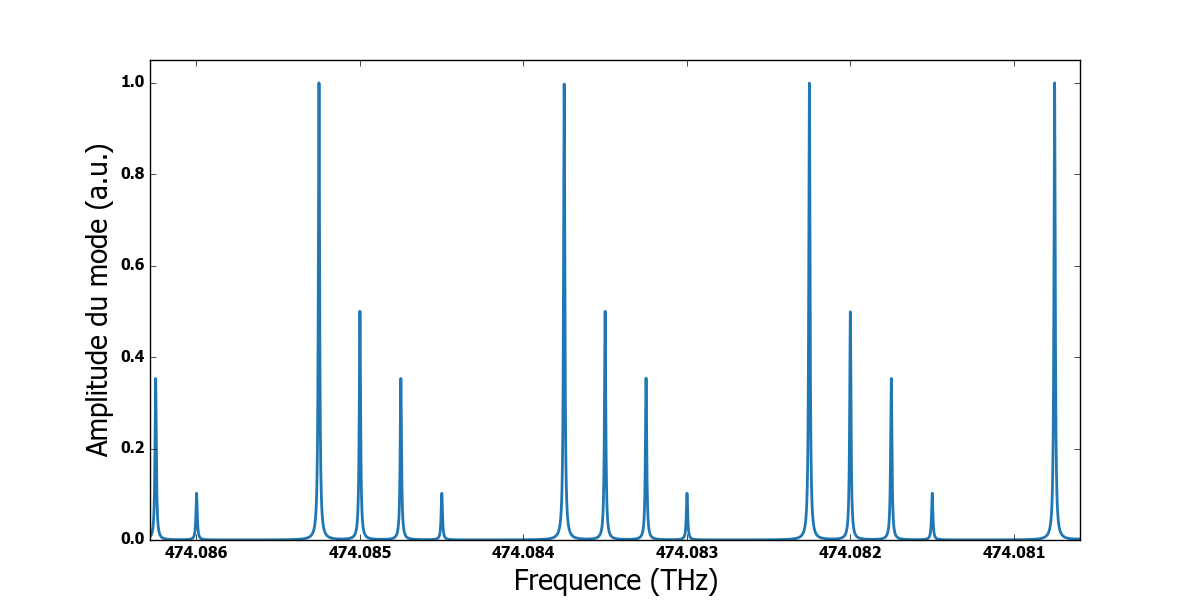
\includegraphics[width=15cm]{pictures/ModeAmplitude.png}
\end{center}
\caption{Spectrographe arbitraire des modes longitudinaux et transverses. L'espacement entre les modes a été calculé pour une cavité ayant les propriétés suivantes : $R_1 = 10\,$m, $R_2 = 20\,$m, $\mathcal{L} = 0.1\,$m, avec une largeur de raie $\delta\nu/\nu = 10^{-8}$.}
\label{fig:modes_long_et_trans}
\end{figure}

La figure~\ref{fig:modes_long_et_trans} présente un exemple arbitraire de spectrographe donnant la répartition des modes en cavité. Dans un laser, il est évidemment nécessaire de de tenir compte de la réponse spectrale du gain du milieu amplificateur pour obtenir le spectre d'émission. 


\chapter{Application : accélération d'électrons par laser}

\section{Introduction}
Le contenu de ce cours est un peu spécial puisqu'il présente une application des lasers qui n'est pas de l'optique, mais à la croisée des chemins entre l'optique, l'interaction laser-matière et l'électrodynamique relativiste. Nous aborderons par conséquent un grand nombre de notions de physique de base, en particulier d'électromagnétisme. Ce support écrit donne les grandes lignes et les concepts essentiels qui vous permettront d'avoir une idée schématique des processus permettant l'accélération d'électrons par laser. 

Comme nous l'avons souligné dans l'introduction, l'essor de l'utilisation des lasers impulsionnels est remarquable : ils ont d'une part peuplé des domaines aussi éloignés que la découpe de tôle et la chirurgie de l'\oe{}il, et ils trouvent d'autre part des applications en recherche fondamentale. Dans un grand nombre de ces activités de recherche, c'est l'intensité crête qui fait l'attractivité des lasers impulsionnels : cette dernière peut atteindre $10^{22}\,\mathrm{W/cm^2}$. L'interaction entre un laser aussi intense et la matière permet d'accéder à des phénomènes physiques dits \textit{relativistes}, c'est-à-dire qu'ils mettent en jeu des énergies cinétiques de l'ordre de l'énergie de masse des particules mises en mouvement par le champ. Pour un électron, cela correspond à une énergie cinétique de l'ordre de $1\,\mathrm{MeV}$. 


Nous appréhenderons les phénomènes fondamentaux permettant l'accélération d'électrons par interaction entre un laser impulsionnel ultra-intense et un gaz moléculaire. Nous commencerons par une brève introduction aux accélérateurs coventionnels et à leurs limitations, ainsi qu'aux raisons pour lesquelles l'accélération par laser peut permettre de dépasser ces limites. Nous décrirons ensuite les phénomènes physiques qui ont lieu dans la matière lorsqu'on l'illumine à des intensités supérieures à $10^{16}\,\mathrm{W/cm^2}$. Nous verrons que l'arrivée de l'impulsion provoque tout d'abord l'ionisation du milieu, et génère ainsi un plasma. Lorsque l'intensité dépasse les quelques $10^{18}\,\mathrm{W/cm^2}$, selon la densité éléctronique du plasma, on peut alors déclencher une excitation d'ondes plasma de forte amplitude donnant lieu à l'accélération d'électrons. Nous discuterons en particulier de ce qu'on appelle le ``régime de la bulle'' dans lequel l'onde plasma est excitée de façon résonante. Elle prend alors un caractère non-linéaire, et le champ éléctrique qui en résulte peut dépasser $100\,\textrm{GV/m}$. Nous verrons alors comment ce champ électrique permet d'accélérer des électrons à des énergies relativistes.

\section{Considérations sur les accélérateurs conventionnels, et limitations}

Le principe de base de l'accélération de particules repose sur la génération d'un champ électrique accélérateur ainsi que sur l'injection d'électrons dans un tel champ. Le tout premier appareil conçu s'apparentant à un accélérateur de particules est le tube de Geissler (ou tube cathodique). Il s'agit d'un tube de verre, contenant une faible pression de gaz, souvent des gaz rares comme le néon ou l'argon, mais aussi d'autres gaz tels que le sodium ou le mercure. De part et d'autre de ce tube sont placées deux électrodes sur lesquelles on applique une haute tension. Le champ éléctrique fort ainsi créé provoque l'ionisation provoque la génération de lumière dont la couleur dépend du gaz utilisé. La haute tension appliquée induit à la fois l'ionisation des atomes ainsi qu'un courant électrique. C'est la recombinaison des électrons avec les ions (et la désexcitation radiative qui s'ensuit) qui produit l'émission de lumière par fluorescence. Lorsque le tube est sous vide poussé, on appelle ce type de dispositif un tube de Crookes (du scientifique anglais W.~Crookes qui est son inventeur). Dans un tube de Crookes, un ratonnement lumineux est aussi émis, mais seulement au niveau de l'anode. Ces rayonnements, à l'époque mystérieux furent nommés rayons cathodiques. En 1897, J.~J.~Thomson (le même que celui du modèle atomique de Thomson !) démontra que ces rayonnement provenaient d'une particule, alors inconnue, qui fut nommée ``électron''. 

C'est en partant de ce principe que Cockcroft and Walton développèrent le tout premier accélérateur de particules lors de leurs travaux avec Rutherford. Il s'agissait d'un accélérateur de protons destiné à l'étude de la structure interne de l'atome. L'accélérateur fut mis en service en mars 1932. Un mois plus tard, Rutherford, Cockcroft et Walton mirent en évidence la première fission atomique artificielle par bombardement de protons sur une cible de lithium. L'énergie des protons à l'époque était de 710$\,\mathrm{keV}$. Ce type d'accélérateur est ce que l'on appelle un accélérateur électrostatique, toujours très utilisé aujourd'hui notamment dans les tubes à rayons X utilisés pour les radiographies médicales. L'énergie des particules issues d'un tel accélérateur est cependant limitée par le champ de claquage (même sous "vide" !) à environ 1$\,\mathrm{MV/m}$. On peut pour certaines applications utiliser des gaz isolants tels que le $\mathrm{SF}_6$ afin de multiplier cette limite par un facteur 30.

Une autre méthode, l'accélération radiofréquence fut inventée par Ising et développée par Wider{\o}e en 1928 (voir Fig.~\ref{fig:wideroe} et Fig.~\ref{fig:acc_dec}. En connectant une série d'électrodes de polarités alternées, on peut arriver à des énergies assez importantes mais sur des dimensions colossales comme le SLAC (l'accélérateur linéaire de Stanford) qui peut accélérer des électrons à 50$\,\mathrm{GeV}$, sur une distance de 3,2$\,\mathrm{km}$ ! En général ce type d'accélérateur est utilisé autour de quelques dizaines de MeV. En principe, ce type d'appareil permet de démultiplier la tension d'alimentation étage après étage, tant que le faisceau (impulsionnel !) est isolé du champ décélérateur (déphasé de $\pi$). On peut faire un calcul simple des dimensions de l'accélérateur pour des énergies non-relativistes : le gain d'énergie après le $n$-ième étage est le suivant~:

\begin{equation}
    E_n=nqU_0\sin\left(\phi_s\right)
    \label{eq:linac_energy}
\end{equation}
où $n$ est le nombre d'étages d'accélération, $q$ est la charge de la particule, $U_0$ la tension d'alimentation et $\phi_s$ la phase relative entre l'impulsion de particules et la tension sinusoïdale. 
Il apparaît clairement que la quantité fondamentale dans cette équation est la longueur des étages d'accélération. Pour une radiofréquence donnée, la longueur de l'étage d'accélération est imposée par la vitesse des particules et la demi-période de l'onde RF. On obtient ainsi que $l_n = v_n\cdot \tau_{RF}/2$. Toujours dans l'approximation classique, l'énergie cinétique de la particule est simplement donnée par $E_{kin} = 1/2mv^2$. En insérant ces expressions dans l'équation~\ref{eq:linac_energy}, on obtient la longueur de l'étage en fonction des paramètres de l'accélérateur~:

\begin{equation}
    l=\frac{1}{\nu_{RF}}\sqrt{\frac{nqU_0\sin{\phi_s}}{2m}}
\end{equation}

Pour des vitesses relativistes, le gain d'énergie n'est évidemment plus linéairement croissant avec le nombre d'étages, et les longueurs des sections deviennent extrêmement longues (l'exemple du SLAC cité précédemment le démontre). 

Afin d'accéder à des énergies encore plus importantes, et pouvant aller jusqu'à quelques $\mathrm{TeV}$, on utilise d'autres structures appelées synchrotrons et anneaux de stockage. L'exemple le plus célèbre est évidemment le LHC au CERN. Le LHC fait 27$\,\mathrm{km}$ de circonférence, et a permis l'accélération de protons à 6.5$\,\mathrm{TeV}$ (actuellement, c'est la plus grande machine au monde). 
Pour plus d'informations sur les accélérateurs, la lecture de l'article de Bernhard Holzer sur les accélérateurs et leur limites \cite{holzer}. 

\begin{figure}[!htbp]
\begin{center}
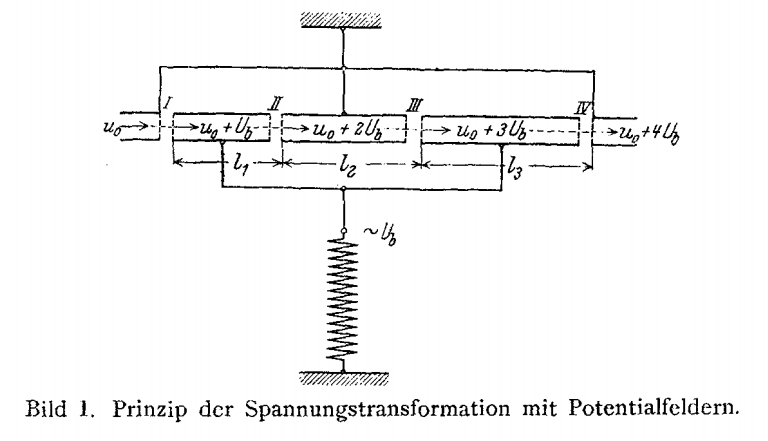
\includegraphics[width=11cm]{pictures/Wideroe.png}
\end{center}
\caption{Accélérateur de Wider{\o}e~\cite{Wideroe1928}}
\label{fig:wideroe}
\end{figure}

\begin{figure}[!htbp]
\begin{center}
\includegraphics[width=8cm]{}
\end{center}
\caption{Champs accélérateur et décélérateur dans un accélérateur radiofréquence}
\label{fig:acc_dec}
\end{figure}

Il est assez clair que l'un des facteurs limitants est la taille des structures accélératrices qui devient monumentale lorsqu'on atteint des vitesses relativistes. C'est le problème que l'accélération laser-plasma pourrait permettre de résoudre. De plus, nous verrons que les propriétés 


\section{L'accélération par interaction laser-plasma}

\subsection{Introduction}

"Puisque la limite des champs accélérateurs est le champ de claquage, utilisons donc un milieu déjà claqué !" Ainsi pourrions nous décrire avec un brin d'humour l'idée de base de l'utilisation des champs présents dans un plasma pour accélérer des électrons. \textit{[Cette dernière remonte d'après \cite{malka} à une intervention de Budker en 1956 \cite{budker} mais dont l'auteure du document présent n'a pu trouver de trace en ligne (peut-être l'article en question se trouve-t-il dans les bibliothèques du CERN ?...)]}  
L'idée de base repose sur le fait qu'un plasma peut accomoder des champs électriques colossaux lorsque les charges libres sont accumulées dans une zone de l'espace, comme dans une onde plasma. 


\medskip

\noindent\fcolorbox{black}{myGray}{%
    \minipage[t]{\dimexpr1\linewidth-2\fboxsep-2\fboxrule\relax}
        \textbf{Calcul d'ordre de grandeur du champ collectif dans un plasma :\\}
          Sachant qu'on a un plasma de densité électronique $10^{19}\,\mathrm{cm^{-3}}$, quelle est la fréquence plasma $\omega_p$ associée~? Que représente-t-elle~? Quelle est la longueur d'onde plasma $\lambda_p$~? Et le vecteur d'onde $k_p$~?\\
          \\
          \begin{itemize}
              \item  $\omega_p = $
              \\\\
              \item  $\lambda_p = $
              \\\\
              \item  $k_p = $
              \\\\
          \end{itemize}
         
          \\\\

          On suppose qu'on excite une telle onde, et que la distribution de la densité électronique est de la forme $\rho(x, y, z) = \rho_0\cos{k_p z}$. Quel est le champ longitudinal $E_z$ maximal dans le milieu~? (On pensera à appliquer le théorème de Gauss)\\
          \\
          \begin{itemize}
              \item  $E_z = $
              \\\\
          \end{itemize}
          \\\\\\\\
    \endminipage}\hfill
    
\medskip

Comment alors générer une telle onde plasma et atteindre les quelques 300$\,$GV/m estimés ci-dessus~? En 1979, Dawson et Tajima proposèrent une idée portée par la technologie en emergence : l'onde plasma pouvait être excitée par laser \cite{tajima}, dans un plasma généré par l'impulsion laser elle-même. 

\subsection{Génération d'un plasma par suppression de barrière de potentiel}

Comme nous l'avons mentionné au tout début de ce chapitre, lorsqu'on focalise un laser intense à quelques $10^{18}\,\mathrm{W/cm^2}$ dans un matériau, les "pieds" de l'impulsion ionisent déjà le milieu. Dans cette section, nous proposons de calculer l'énergie requise pour qu'un faisceau gaussien homogène focalisé dont le waist $w_0$ est de $10\,\mathrm{\mu m}$, et de durée d'impulsion $30\,\mathrm{fs}$ ionise le premier niveau de l'atome d'Hélium. 

Commençons par estimer le champ électrique nécessaire pour ioniser l'atome d'Hélium. Dans un atome, les électrons sont liés au noyau par le potentiel coulombien (voir Figure~\ref{fig:potentiel} résultant de la combinaison des charges du noyau et des charges des électrons du nuage atomique le cas échéant. Ce potentiel s'écrit~:
\begin{equation}
    V(r)=-\frac{Z*e^2}{4\pi\epsilon_0r}
\end{equation}
où $Z*$ est le numéro atomique effectif (il prend en compte l'écrantage du champ du noyau par les électrons), $e$ est la charge électronique élémentaire, et $r$ est la position radiale. Il existe une énergie $V_i$ pour laquelle un électron piégé dans un tel potentiel n'est plus lié. C'est ce qu'on appelle l'énergie d'ionisation. 

Dans les fréquences optiques, le moment dipolaire magnétique est négligeable par rapport au moment dipolaire électrique. La contribution au potentiel du laser se limite donc à son champ électrique $E_0$. On a alors~:

\begin{equation}
    V(r)=-\frac{Z*e^2}{4\pi\epsilon_0r}-eE_0z
\end{equation}

La figure~\ref{fig:potentiel} montre que le champ extérieur abaisse la barrière de potentiel. Lorsque cette dernière passe en-dessous de l'énergie de liaison $V_i$, on a ionisation par suppression de barrière. Pour calculer ce champ, on calcule le maximum du potentiel (abscisses positives sur la figure~\ref{fig:potentiel}) au point $z_M$ tel que $\left(\partial V/\partial r\right)_{r_M}=0$. Ce maximum se situe en $r_M=\left(\frac{Z*e}{4\pi\epsilon_0E}\right)^{1/2}$, où le potentiel vaut~:

\begin{equation}
    V(r_M)=2e\left(\frac{Z*eE}{4\pi\epsilon_0}\right)^{1/2}
    \label{eq:max_potentiel}
\end{equation}

\begin{figure}[!htbp]
\begin{center}
\includegraphics[width=8cm]{}
\end{center}
\caption{Potentiel coulombien, effet du champ laser sur le potentiel}
\label{fig:potentiel}
\end{figure}

L'équation~\ref{eq:max_potentiel} nous permet de calculer le champ $E_{sb}$ tel que $V(r_M)<V_i$ qui correspond au champ électrique seuil pour atteindre le régime de suppression de barrière : $E_{sb}=\frac{\pi\epsilon_0V_i^2}{Z*e^3}$. Le paramètre mesuré lors d'expériences est l'intensité du champ, qui correspond à une densité surfacique de puissance, et s'exprime en fonction du champ électrique~:~$I=\frac{\epsilon_0cE^2}{2}$. On obtient alors l'intensité de suppression de barrière~:

\begin{equation}
    I_{sb}\left[\mathrm{J/s/m^2}\right]=\frac{\pi^2c\epsilon_0^3V_i^4}{2e^6Z*^2}
    \label{eq:Isb}
\end{equation}

Dans l'approximation du champ central, le champ subi par l'électron le plus périphérique est écranté par $Z-1$ électrons, on obtient alors $Z* = Z-(Z-1) = 1$. En insérant les valeurs des constantes fondamentales dans l'équation~\ref{eq:Isb}, on trouve la valeur de l'intensité dans des unités d'expérimentateur (en $\mathrm{W/cm^2}$)~:

\begin{equation}
    I_{sb}(\mathrm{W/cm^2})=4\times10^9\frac{V_i^4\mathrm{(eV)}}{Z*^2}
\end{equation}

Les valeurs des énergies d'ionisation sont des données expérimentales mesurées disponibles sur des bases de données de référence (voir par exemple https://physics.nist.gov/PhysRefData/ASD/ionEnergy.html~) et on peut alors facilement calculer l'intensité laser nécessaire pour ioniser un atome donné. Pour l'Hélium, les énergies d'ionisation sont de $\approx 24.54\mathrm{eV}$ et $\approx 54.42\mathrm{eV}$. On calcule alors les intensités d'ionisation $I_1=1.45\times10^{15}\,\mathrm{W/cm^2}$ et $I_2=8.77\times10^{15}\,\mathrm{W/cm^2}$. \textit{[On peut faire la même chose pour l'azote et voir pour quelle intensité on peut faire un plasma dans l'air... Rendez-vous à la visite de labo~!]}

Nous pouvons à présent répondre à la question posée en début de section, à savoir, si notre impulsion fait $30\,\mathrm{fs}$ de durée, et est focalisée sur un waist de $10\,\mathrm{\mu m}$, quelle est l'énergie nécessaire pour ioniser l'Hélium~?

Faisons tout d'abord un calcul d'ordre de grandeur pour aiguiser notre intuition. L'intensité est une densité surfacique de puissance. Estimons tout d'abord la puissance instantanée $P$ d'une impulsion d'énergie $U$ et de durée à mi-hauteur $\tau$ par $P = U/\tau$ (Nous avons alors de $\mathrm{J/s}$). Puis, supposons une distribution plate de l'énergie sur un disque de rayon $w_0$. On a une surface $S=\pi w_0^2$, et donc une intensité $I = P/S = U/(\tau S)$. On obtient alors que $137\,\mathrm{\mu J}$ suffisent à ioniser le premier niveau de l'Hélium en première approximation. 

Afin d'affiner cette estimation, revenons à l'expression du mode fondamental d'un champ électromagnétique gaussien dans le plan focal, c'est-à-dire en $z=0$ (Eq.~\ref{eq:HermiteGauss})~:

\begin{equation}
    E(r)=E_0\mathrm{e}^{-\frac{r^2}{w_0^2}}
\end{equation}

On déduit alors l'intensité (en W/cm$^2$ ou J/s/cm$^2$)~:

\begin{equation}
    I(r)=\frac{E_0^2}{2\eta}\mathrm{e}^{-\frac{2r^2}{w_0^2}}
\end{equation}

Si on suppose une disribution temporelle gaussienne de l'impulsion de largeur à 1/e$^2$ égale à $\tau$, on peut alors écrire~:
\begin{equation}
    I(r, t)=\frac{E_0^2}{2\eta}\mathrm{e}^{-\frac{2r^2}{w_0^2}}\mathrm{e}^{-\frac{t^2}{\tau^2}}
\end{equation}

où $\eta = 377\,\mathrm{\Omega}$ est l'impédance caractéristique du vide. La puissance $P(t)$ du faisceau (en W ou J/s) est donnée par~: 
\begin{equation}
    P(t)=\int  r I(r, t)d\theta dr
\end{equation}
et l'énergie $U$ par~:
\begin{equation}
    U=\int  r I(r)d\theta dr dt
\end{equation}

En utilisant les intégrales gaussiennes connues $\int \mathrm{e}^{-ax^2} dx = \sqrt{\frac{\pi}{a}}$ et $\int x^n\mathrm{e}^{-ax^2} dx = \frac{\Gamma(\frac{n+1}{2})}{2a^{\frac{n+1}{2}}}$, on obtient un facteur $\frac{\sqrt{\pi}}{2}$ avec notre estimation "naïve". Une énergie $U = 137\frac{\sqrt{\pi}}{2}\approx 120\,\mathrm{\mu J}$ est donc suffisante pour ioniser le premier niveau de l'Hélium. 

\medskip

\noindent\fcolorbox{black}{myGray}{%
    \minipage[t]{\dimexpr1\linewidth-2\fboxsep-2\fboxrule\relax}
        \textbf{Et pour faire un plasma dans l'air ?\\}
          
            \vspace{40 mm}
       
    \endminipage}\hfill
    
\medskip

Comme vous l'avez appris dans votre cours de mécanique quantique, il existe aussi une probablitité non nulle d'ionisation, même si la barrière de potentiel n'est pas complètement supprimée. C'est ce qu'on appelle l'effet tunnel. Pour plus de détails à ce sujet, veuillez vous référer à votre cours PA101.

\subsection{Excitation d'ondes plasma}

Nous allons à présent nous intéresser au mouvement collectif des électrons dans le plasma en présence d'un champ électromagnétique fort. Cette partie du cours de la physique des plasmas plutôt que de la physique des lasers, et les démonstrations qui suivent ne font pas partie des choses à savoir pour l'examen. Elles apporteront un peu plus de profondeur à votre compréhension de l'interaction lumière-matière pour des champs intenses. On soulignera aussi que la physique contemporaine se situe souvent au croisement entre plusieurs domaines. Dans ce cours vous trouverez évidemment de l'électromagnétisme, mais aussi de la mécanique des fluides et un peu de physique semi-classique.

\subsubsection{Mouvement d'une tranche d'électrons dans un plasma}

On veut tout d'abord connaître le mouvement d'un ensemble d'électrons dans un plasma de densité $n_0$, en présence d'un champ électrique. On supposera que les ions sont lourds, et que par conséquent leurs déplacements sont négligeables par rapport à ceux des électrons. A l'équilibre, la densité ionique et la densité électronique sont homogènes. De plus, on supposera que le mouvement thermique de électrons est négligeable. Cela n'est pas nécéssairement le cas, mais pour notre cas particulier, l'énergie cinétique des électrons mis en mouvement par le laser est bien plus élevée que l'énergie thermique et on peut donc supposer qu'il n'y a pas de collisions. 


\begin{figure}[!htbp]
\begin{center}
\includegraphics[width=8cm]{}
\end{center}
\caption{Déplacement d'une tranche d'électrons dans le plasma}
\label{fig:osc_plas}
\end{figure}

Lorsque les électrons sont déplacés de leur position d'équilibre par un champ électrique externe (tel qu'un champ laser) d'une quantité $x$ (voir Figure~\ref{fig:osc_plas}), ils subissent une force de rappel $F=-e E_x$ dûe au champ électrostatique qui résulte de ce déplacement. On peut alors très simplement écrire l'équation du mouvement en 1D de ces électrons~: 

\begin{equation}
    m_e\frac{d^2 x}{dt^2}=-eE_x(x)
\end{equation}

Si on considère la variation de la densité de charge en fonction de la position représentée figure~\ref{fig:osc_plas} et qui découle de la conservation de la charge, on peut appliquer la Loi de Gauss $\nabla\cdot\textbf{E}=-\frac{e n_0}{\epsilon_0}$ que l'on intègre de 0 à $x$~: 

\begin{equation}
    E_x(x) = en_0\frac{x}{\epsilon_0}
    \label{eq:chp_E}
\end{equation}

On obtient alors l'équation du mouvement des électrons~:
\begin{equation}
    \frac{d^2x}{dt^2}+\frac{n_0e^2}{\epsilon_0 m_e} x =0
\end{equation}

La solution à cette équation est une oscillation harmonique de pulsation $\omega_p = \sqrt{\frac{n_0 e^2}{\epsilon_0 m_e}}$ que l'on appelle la pulsation de Langmuir. 
Soumis à une perturbation, les électrons suivent donc, dans le régime linéaire, un mouvement oscillant collectif $x(t) = x_0\cos(\omega_p t +\theta_0)$. 
Cette onde électronique est ce que l'on appelle une onde de sillage lorsqu'elle est excitée par un champ laser. Cet nom est donnée par analogie à l'onde générée dans le sillage d'un bateau (Fig.~\ref{fig:sillage})

\begin{figure}[!htbp]
\begin{center}
\includegraphics[width=10cm]{pictures/Fjordn_surface_wave_boat.png}
\end{center}
\caption{Onde de sillage. \textcopyleft Edmont [CC BY-SA 3.0 (https://creativecommons.org/licenses/by-sa/3.0) }
\label{fig:sillage}
\end{figure}



\subsubsection{Mouvement collectif des électrons, approche Hamiltonienne}

La mécanique Hamiltonienne est l'approche la plus élégante d'étudier le mouvement des électrons dans l'onde plasma. Comme la mécanique Newtonienne, elle permet d'établir les équations du mouvement d'un système soumis à un ensemble de forces, et repose, pour faire simple, sur la conservation de l'énergie. Dans le cas de notre tranche d'électrons perturbés, on a une énergie cinétique $\frac{p_x^2}{2m_e}$ et une énergie potentielle électrostatique $\Phi_E$ que l'on peut déduire du champ électrique établi dans la section précédente (équation~\ref{eq:chp_E}). On sait tout d'abord que la force électrostatique est conservative, le champ est donc le gradient du potentiel. De plus, l'énergie électrostatique est le produit de la charge et du potentiel, on a donc~:

\begin{equation}
    \textbf{E}=-\nabla V_E \quad \mathrm{et} \quad \Phi_E=-eV_E
\end{equation}

d'où on déduit $\Phi_E=\frac{e^2n_0}{\epsilon_0}x^2$, ce qui nous permet d'écrire l'Hamiltonien du système~:

\begin{align}
    H &= E_K + \Phi_E \\
      &= \frac{p^2}{2m_e}+\frac{e^2n_0}{2\epsilon_0}x^2
      \label{eq:hamiltonien}
\end{align}
On trouve l'évolution temporelle du système en mécanique Hamiltonienne par les relations suivantes~:

\begin{equation}
    \frac{dp}{dt}=-\frac{\partial H}{\partial q}, \quad \frac{dq}{dt}=\frac{\partial H}{\partial p}
\end{equation}

où $p$ est la quantité de mouvement et $q$ la position. En appliquant ces relations au Hamiltonien~\ref{eq:hamiltonien}, on obtient alors~:

\begin{eqnarray}
        \frac{dp(t)}{dt}&=-\frac{n_0e^2}{\epsilon_0}x(t)\\
        \frac{dx(t)}{dt}&=-\frac{p(t)}{m_e}
\end{eqnarray}
n obtient alors le système d'équations~:

\begin{equation}
    H=\sqrt{1+u_z^2}-e\phi(z-v_pt)
\end{equation}
que l'on peut dériver et réarranger afin d'obtenir les équations différentielles pour la position $x$ et la quantité de mouvement $p$~:

\begin{eqnarray}
        \frac{d^2x(t)}{dt^2} +\frac{n_0e^2}{m_e\epsilon_0}x(t)= 0\\
        \frac{d^2p(t)}{dt^2} +\frac{n_0e^2}{m_e\epsilon_0}p(t)= 0
\end{eqnarray}

que l'on peut résoudre avec la condition initiale $x(0)=x_0$ et $p(0)=0$. En utilisant $\omega_0^2=\frac{n_0e^2}{\epsilon_0}$ a alors le couple d'équations paramétriques suivant~:

\begin{eqnarray}
       x(t)&=x_0\cos{\omega_0 t} \\
       p(t)&=-m_ex_0\omega_0\sin{\omega_0 t}
\end{eqnarray}

En écrivant $x^2(t)+\frac{p^2(t)}{m\omega_0}=x_0^2\cos{\omega_0t}+x_0^2\sin{\omega_0t}=x_0^2$, on peut alors facilement représenter $\frac{p^2(t)}{m\omega_0}$ en fonction de $x$, voir figure~\ref{fig:espace_phases}. C'est ce qu'on appelle l'espace des phases. Cet outil nous sera très utile dans l'analyse des trajectoires des électrons dans le plasma. 


\begin{figure}[!htbp]
\begin{center}
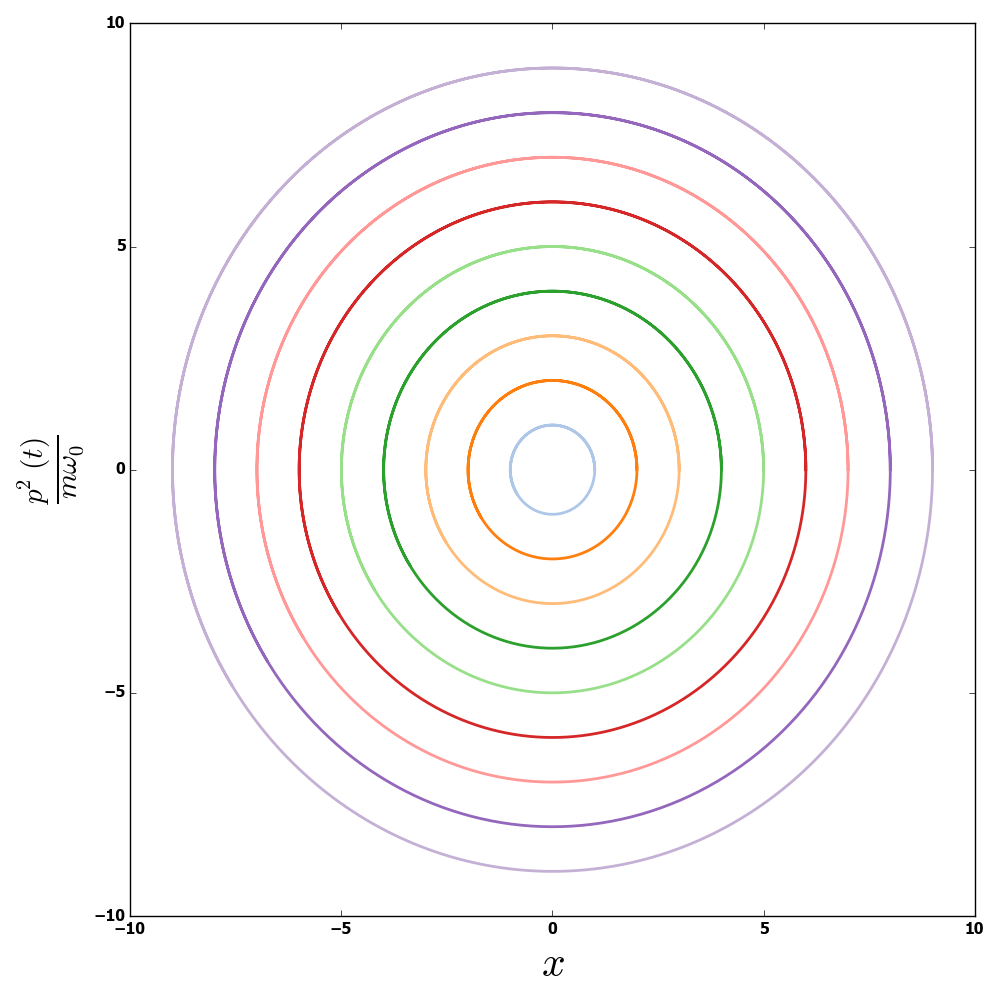
\includegraphics[width=8cm]{pictures/simple_phase_space.png}
\end{center}
\caption{Espace des phases pour un oscillateur harmonique non-amorti}
\label{fig:espace_phases}
\end{figure}


\medskip

\noindent\fcolorbox{black}{myGray}{%
    \minipage[t]{\dimexpr1\linewidth-2\fboxsep-2\fboxrule\relax}
        \textbf{Et pour un oscillateur amorti ?\\}
          
            \vspace{40 mm}
       
    \endminipage}\hfill
    
\medskip

\subsubsection{Mouvement des électrons dans l'onde plasma}
Nous venons de voir que lorsqu'un plasma est perturbé (par un champ externe dans notre cas), il est mis en mouvement et oscille à la pulsation de Langmuir $\omega_p = \sqrt{\frac{n_0 e^2}{\epsilon_0 m_e}}$. Dans ce modèle très simple, les électrons oscillent mais n'obtiennent aucune quantité de mouvement longitudinale. Afin de modéliser les trajectoires des électrons, et de montrer qu'il existe des conditions sous lesquelles un électron peut être piégé dans l'onde plasma et suivre ainsi l'impulsion laser, on peut considérer l'Hamiltonien en 1D d'un électron soumis d'une part au champ laser et d'autre part au potentiel électrostatique $\phi$ dû à l'onde plasma elle-même~: 

\begin{equation*}
    H=m_ec^2\sqrt{1+\frac{p_z^2}{m_e^2c^2}+\frac{p_\perp^2}{m_e^2c^2}}-e\Phi(z-v_pt)
\end{equation*}

Le premier terme représente l'énergie de masse de l'électron et son énergie cinétique, et le deuxième terme, son énergie potentielle. Cette dernière, dans le cas d'une onde plasma harmonique, est une onde sinusoïde qui se déplace à la vitesse de phase $v_p$. Afin de simplifier les notations, on normalise cet Hamiltonien en utilisant les variables $u_z=\frac{p_z}{m_ec}$ et $\phi = \frac{e\Phi}{m_ec^2}$~:

\begin{equation}
    H=\sqrt{1+u_z^2+u_\perp^2}-\phi(z-v_pt)
\end{equation}

Cet Hamiltonien dépend du temps et de la position, mais les deux sont couplés par la vitesse, ce qui se traduit par une dépendance en $\zeta = z-v_pt$, on peut alors effectuer la transformation canonique de l'Hamiltonien $(z, u_z)\rightarrow(\zeta, u_z)$. En utilisant la fonction génératrice du second type $F_2(z, u_z)=u_z(z-v_pt)$ vérifiant les deux conditions~:

\begin{eqnarray*}
    \frac{\partial F_2}{\partial u_z}&=\zeta\\
    \frac{\partial F_2}{\partial z}&=u_z
\end{eqnarray*}

On peut ainsi simplifier l'Hamiltonien en utilisant la relation $H' = H+\frac{1}{c}\frac{\partial F_2}{\partial t}$~:

\begin{equation}
    H'=\sqrt{1+u_z^2+u_\perp^2}-\phi(\zeta)-\frac{v_p}{c}u_z
\end{equation}

En définissant $\beta=v_p/c$, on obtient l'Hamiltonien que nous utiliserons pour notre analyse des trajectoires~:

\begin{equation}
    H'=\sqrt{1+u_z^2+u_\perp^2}-\phi(\zeta)-\beta_p u_z
\end{equation}

En une dimension, l'Hamiltonien ne varie pas en fonction de $r_\perp$, c'est-à-dire $\partial H/\partial r_\perp = 0$. On peut en déduire que la somme de la composante transverse de la quantité de mouvement $u_\perp$ et de l'amplitude du laser (purement transverse en 1D) doit être constante~:~ $u_\perp(\zeta) - a(\zeta) = \mathrm{cste}$, où $a(\zeta)$ est ce qu'on appelle le potentiel vecteur normalisé. 

\textit{[NDA~:~Pour ceux d'entre vous qui n'ont jamais rencontré le potentiel vecteur, sachez simplement qu'il s'agit d'un potentiel duquel le champ électomagnétique dérive (de la même manière qu'on a $\textbf{E} = -\nabla V$ où $\textbf{E}$ est le champ électrique et $V$ le potentiel duquel le champ dérive, on a $\textbf{B} = \nabla\times\textbf{A}$ avec $\textbf{B}$ le champ magnétique et $\textbf{A}$ le potentiel vecteur.]}


Par conservation de l'énergie, si un électron est placé en $\zeta_0$ avec une énergie cinétique $\gamma_0$ à $t=0$, son Hamiltonien $H_0$ est donc une constante du mouvement. En résolvant l'équation polynômiale du second ordre pour $u_z$, on obtient~:

\begin{equation}\label{eqsol}
u_z(\zeta) = \beta_p\gamma_p^2(H_0+\phi(\zeta))\pm\gamma_p\sqrt{\gamma_p^2(H_0+\phi(\zeta))^2-\gamma\perp^2}
\end{equation}

Cette équation décrit les trajectoires des électrons dans l'onde de sillage dans l'espace des phases $(\zeta, u_z)$ en fonction de leur condition initiale $H_0$. 

Afin de pouvoir calculer ces trajectoires, il est nécessaire de connaître le potentiel électrostatique $\phi$ de l'onde de sillage. On peut montrer qu'en une dimension, ce potentiel est régi par l'équation suivante~:

\begin{equation}
    \frac{\partial^2 \phi}{\partial \zeta ^2 }\approx\frac{k_p^2}{2}\left(\frac{1+a^2/2}{(1+\phi)^2}-1\right)
    \label{eq:1Dnonlinear}
\end{equation}
où $a$ est \textit{grosso modo} l'amplitude du potentiel issu du champ laser (on l'appelle le "potentiel vecteur normalisé"). Pour des lasers intenses, on a $a>1$. Pour notre exemple, nous allons prendre $a=3$. En résolvant l'équation~\ref{eq:1Dnonlinear} numériquement, on peut alors tracer le potentiel électrostatique $\phi$ et le champ électrique $E$ qui en dérive en fonction de notre variable d'espace-temps $\zeta$ qui se déplace à la vitesse de groupe de l'impulsion laser (voir Fig.~\ref{fig:1D_pot_field}). 


\begin{figure}[!htbp]
\begin{center}
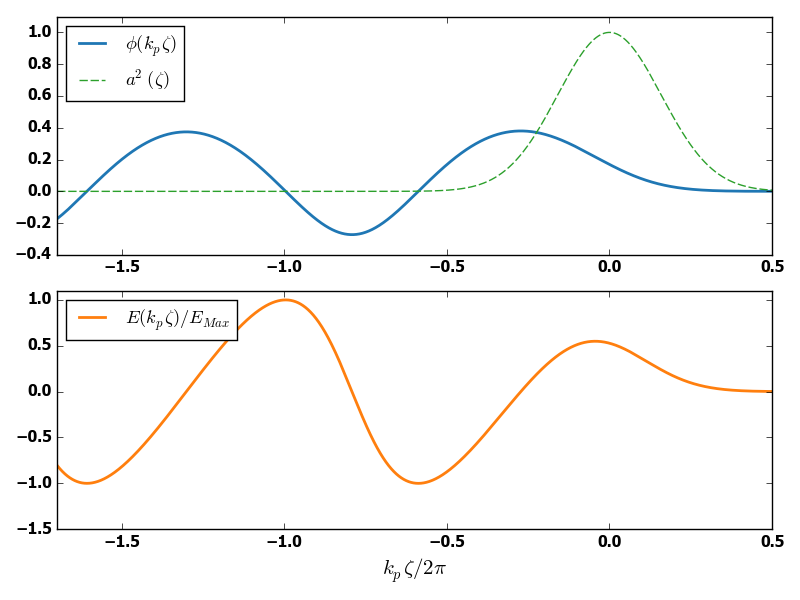
\includegraphics[width=9cm]{1D_Field_and_Potential.png}
\end{center}
\caption{Potentiel $\phi$ et champ électrique $E$ de l'onde de sillage}
\label{fig:1D_pot_field}
\end{figure}

Nous pouvons alors tracer les trajectoires des particules dans ce potentiel dans l'espace des phases~$(\gamma, k_p\zeta)$.


Nous observons deux types de trajectoires dans cet espace des phases ainsi qu'une trajectoire limite (en rouge) que l'on appelle la séparatrice, et qui délimite les trajectoires piégées des trajectoires non-piégées. La trajectoire en noir représente les électrons qui étaient au repos ($u_z = 0$) à l'arrivée de l'impulsion laser. Ces électrons oscillent dans l'onde plasma un peu comme une bouée oscille sur les vagues : sa quantité de mouvement longitudinale est centrée autour de zéro (on a tracé $u_z+1$ en échelle logarithmique par souci de lisibilité). Les électrons de faible énergie oscillent eux aussi, mais avec une quantité de mouvement moyenne non-nulle, jusqu'à ce que l'énergie soit suffisante pour que ces électrons soient piégés dans l'onde plasma. Les trajectoires fermées correspondent ainsi à des électrons de vitesse longitudinale suffisamment importante pour "surfer" le champ accélérateur et ainsi suivre l'impulsion laser à la vitesse de groupe. C'est ce phénomène de piégeage dans l'onde plasma qui permet l'accélération de particules par laser. 

\begin{figure}[!htbp]
\begin{center}
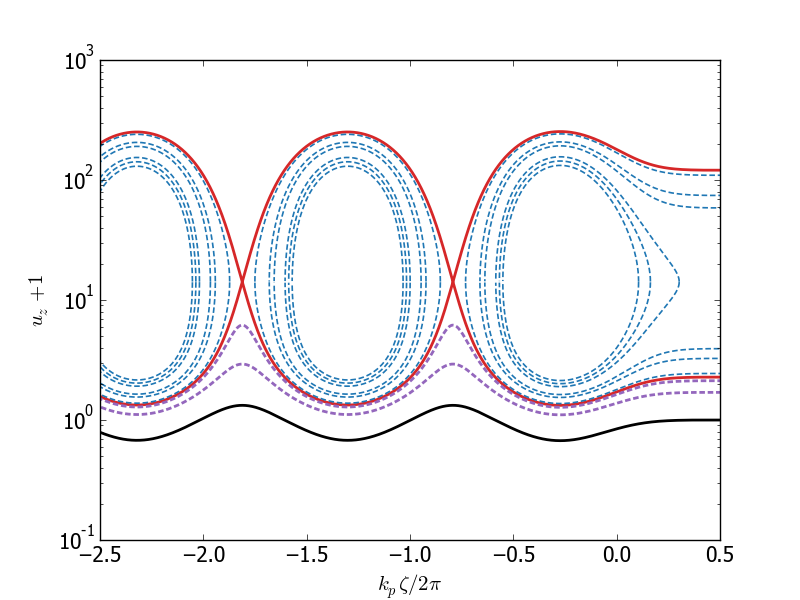
\includegraphics[width=12cm]{pictures/trajectories.png}
\end{center}
\caption{Trajectoires des électrons dans l'onde de sillage. En noir : trajectoire des électrons à l'arrêt devant l'impulsion laser. En rouge : trajectoire limite, dite séparatrice. En bleu : trajectoires d'électrons pégés dans l'onde plasma. }
\label{fig:trajectories}
\end{figure}

\subsubsection{Une expérience d'accélération laser-plasma au laboratoire d'optique appliquée}


\printbibliography[title={Bibliographie}]



%\bibliographystyle{plain}
%\bibliography{bibliography.bib}
\end{document}